\RCS$Revision: 366267 $
\RCS$HeadURL: svn+ssh://bainbrid@svn.cern.ch/reps/tdr2/papers/SUS-14-006/trunk/SUS-14-006.tex $
\RCS$Id: SUS-14-006.tex 366267 2016-09-02 13:36:53Z bainbrid $

\newlength\cmsFigWidth
\ifthenelse{\boolean{cms@external}}{\setlength\cmsFigWidth{0.98\columnwidth}}{\setlength\cmsFigWidth{0.8\textwidth}}
\ifthenelse{\boolean{cms@external}}{\providecommand{\cmsLeft}{top}}{\providecommand{\cmsLeft}{left}}
\ifthenelse{\boolean{cms@external}}{\providecommand{\cmsRight}{bottom}}{\providecommand{\cmsRight}{right}}

\newcommand{\cls}{\text{CL$_s$}\xspace}
\newcommand{\scalht}{\ensuremath{H_\text{T}}\xspace}
\newcommand{\HTmiss}{\ensuremath{H_\text{T}^\text{miss}}\xspace}
\newcommand{\dht}{\ensuremath{\Delta\scalht}\xspace}
\newcommand{\alphat}{\ensuremath{\alpha_\mathrm{T}}\xspace}
\newcommand{\njet}{\ensuremath{N_{\text{jet}}}\xspace}
\newcommand{\njetlow}{\ensuremath{2 \leq \njet \leq 3}\xspace}
\newcommand{\njethigh}{\ensuremath{\njet \geq 4}\xspace}
\newcommand{\nb}{\ensuremath{N_{\PQb}}\xspace}
\newcommand{\mj}{\ensuremath{\mu + \text{jets}}\xspace}
\newcommand{\mmj}{\ensuremath{\mu\mu + \text{jets}}\xspace}
\newcommand{\gj}{\ensuremath{\gamma + \text{jets}}\xspace}
\newcommand{\wjets}{\ensuremath{\PW + \text{jets}}\xspace}
\newcommand{\zjets}{\ensuremath{\cPZ + \text{jets}}\xspace}
\newcommand{\znunujets}{\ensuremath{\cPZ \to \cPgn\cPagn + \text{jets}}\xspace}
\newcommand{\znunu}{\ensuremath{\cPZ \to \cPgn\cPagn}\xspace}
\newcommand{\zmumujets}{\ensuremath{\cPZ \to \mu\mu + \text{jets}}\xspace}
\newcommand{\dphi}{\ensuremath{\Delta\phi^{*}_\text{min}}\xspace}
\newcommand{\dm}{\ensuremath{\Delta m}\xspace}
\newcommand{\alphatmin}{\ensuremath{\alphat^\text{min}}\xspace}
\newcommand{\mhtmet}{\ensuremath{\HTmiss / \ETmiss}\xspace}
\newcommand{\ffbp}{\ensuremath{f{\bar{f}'}}\xspace}

\cmsNoteHeader{SUS-14-006}

\title{Search for top squark pair production in
  compressed-mass-spectrum scenarios in proton-proton collisions at
  $\sqrt{s} = 8\TeV$ using the \alphat variable}

\date{\today}

\abstract{An inclusive search is performed for supersymmetry in final
  states containing jets and an apparent imbalance in transverse
  momentum, \ptvecmiss, due to the production of unobserved weakly
  interacting particles in pp collisions at a centre-of-mass energy of
  8\TeV. The data, recorded with the CMS detector at the CERN LHC,
  correspond to an integrated luminosity of 18.5\fbinv. The
  dimensionless kinematic variable \alphat is used to discriminate
  between events with genuine \ptvecmiss associated with unobserved
  particles and spurious values of \ptvecmiss arising from jet energy
  mismeasurements. No excess of event yields above the expected
  standard model backgrounds is observed. The results are interpreted
  in terms of constraints on the parameter space of several simplified
  models of supersymmetry that assume the pair production of top
  squarks. The search provides sensitivity to a broad range of top
  squark ($\PSQt$) decay modes, including the two-body decay $\PSQt
  \to \PQc \PSGczDo$, where \PQc is a charm quark and $\PSGczDo$ is
  the lightest neutralino, as well as the four-body decay $\PSQt \to
  \PQb \ffbp \PSGczDo$, where \PQb is a bottom quark and $f$ and
  $\bar{f}'$ are fermions produced in the decay of an intermediate
  off-shell W boson. These modes dominate in scenarios in which the
  top squark and lightest neutralino are nearly degenerate in
  mass. For these modes, top squarks with masses as large as 260 and
  230\GeV are excluded, respectively, for the two- and four-body
  decays.}

\hypersetup{
  pdfauthor={M. Baber, R. Bainbridge, O. Buchmueller, D. Burton,
    M. Citron, A. Elwood, Y. Eshaq, H. Flaecher, A. Garcia-Bellido,
    E. Laird, K. Lo, C. Lucas, J. Marrouche, Z. Meng, T. Sakuma,
    D. Smith, and A. Tapper},
  pdftitle={Search for top squark pair production in
    compressed-mass-spectrum scenarios in proton-proton collisions at
    sqrt(s) = 8 TeV using the alphaT variable},
  pdfsubject={CMS},
  pdfkeywords={CMS, physics, SUSY, jets, missing transverse momentum,
    alphaT} 
}

\maketitle

\section{Introduction}

The standard model (SM) is widely regarded as an effective
approximation, valid at low energies, of a more complete theory of
particle interactions, such as supersymmetry (SUSY)~\cite{ref:SUSY-1,
  ref:SUSY0, ref:SUSY1, ref:SUSY2, ref:SUSY3, ref:SUSY4,
  ref:hierarchy1, ref:hierarchy2}, which would supersede the SM at
higher energy scales. A realisation of SUSY with TeV-scale
third-generation squarks is motivated by the cancellation of
quadratically divergent loop corrections to the mass of the Higgs
boson~\cite{ref:atlashiggsdiscovery, ref:cmshiggsdiscoverylong}
avoiding the need for significant fine tuning~\cite{ref:hierarchy1,
  ref:hierarchy2, ref:barbierinsusy}. In R-parity-conserving
SUSY~\cite{Farrar:1978xj}, supersymmetric particles (sparticles) such
as squarks and gluinos are produced in pairs and decay to the lightest
stable supersymmetric particle (LSP), which is generally assumed to be
a weakly interacting and massive neutralino, $\PSGczDo$. A
characteristic signature of these events is a final state with jets
accompanied by an apparent, significant imbalance in transverse
momentum, \ptvecmiss, due to unobserved $\PSGczDo$ particles that can
carry substantial momentum.

The lack of evidence to date for SUSY at the CERN LHC has led to the
careful consideration of regions of the SUSY parameter space that have
a relatively weak coverage in the experimental programme.  One such
class of models is that of compressed mass spectra, in which the LSP
lies close in mass to the parent sparticle produced in the collisions.
Models in which both the top squark ($\PSQt$) and neutralino LSP are
light and nearly degenerate in mass are phenomenologically well
motivated~\cite{Boehm:1999tr,Boehm:1999bj,Balazs:2004bu,
  Martin:2007gf,
  Martin:2007hn,Carena:2008mj,Grober:2014aha,Grober:2015fia}.  For a
mass splitting $\dm = m_{\PSQt} - m_{\PSGczDo} < m_{\PW}$, where
$m_{\PW}$ is the mass of the W boson, the decay modes available to the
top squark are either loop-induced, flavour-changing neutral current
decays to a charm (c) quark and a neutralino, $\PSQt \to
\PQc\PSGczDo$, or four-body decays, $\PSQt \to {\PQb \ffbp} \PSGczDo$,
where b is a bottom quark with $f$ and ${\ffbp}$ fermions from, for
example, an off-shell W boson decay. Improved experimental acceptance
for systems with compressed mass spectra can be achieved by requiring
the sparticles to be produced in association with jets from
initial-state radiation (ISR). The sparticle decay products from these
systems can be Lorentz boosted to transverse momenta within the
experimental acceptance if they recoil against a sufficiently high-\pt
jet from ISR. This topology is exploited by searches that consider
$\text{``monojet''} + \ptvecmiss$ final states~\cite{atlas-13,
  atlas-6, cms-9}. The reliance on ISR is reduced for systems with
larger \dm, as in this case the sparticle decay products can have
sufficiently large values of \pt to lie within the experimental
acceptance even without the Lorentz boost from ISR.

This letter presents an inclusive search for the pair production of
massive coloured sparticles in final states with two or more energetic
jets and \ptvecmiss in pp collisions at $\sqrt{s} = 8\TeV$. The data
correspond to an integrated luminosity of $18.5 \pm
0.5\fbinv$~\cite{lumi} collected with the CMS detector at the LHC. The
search is based upon a kinematic variable \alphat, described in
Section~\ref{sec:alphat}, which offers powerful discrimination against
SM multijet production, and adheres to a strategy of maximising
experimental acceptance through the application of loose selection
requirements to provide sensitivity to a wide range of SUSY
models. Previous versions of this search were reported at $\sqrt{s} =
7\TeV$~\cite{RA1Paper, RA1Paper2011, RA1Paper2011FULL}, and for an
initial sample of data corresponding to 11.7\fbinv at
$8\TeV$~\cite{RA1Paper2012}. Other LHC searches for manifestations of
SUSY in all-jet final states are presented in Refs.~\cite{atlas-0,
  atlas-1, atlas-2, atlas-3, atlas-4, atlas-5, atlas-11, atlas-7,
  atlas-8, atlas-9, atlas-10, atlas-12, cms-1, cms-2, cms-3, cms-4,
  cms-8,cms-11,cms-5, cms-6, cms-7, cms-10, cms-12, cms-13, atlas-13,
  atlas-6, cms-9}.
%Recent searches for top squark production in leptonic final states can
%be found in Refs.~\cite{Aad:2015pfx} (and references therein)
%and~\cite{Khachatryan:2016pup}.

The search makes use of the number of reconstructed jets per event
(\njet), the number of these jets identified as originating from b
quarks (\nb), and the sum of the transverse energies of these jets
(\scalht), where the transverse energy of a jet is given by $\ET =
E\sin\theta$, with $E$ the energy of the jet and $\theta$ its polar
angle with respect to the beam axis. The three discriminants provide
sensitivity to different production mechanisms of massive coloured
sparticles at hadron colliders (\ie squark-squark, squark-gluino, and
gluino-gluino), to a large range of mass splittings between the parent
sparticle and the LSP, and to third-generation squark signatures.
Interpretations of the analysis are provided in the parameter space of
a variety of simplified models~\cite{Alwall:2008ag, Alwall:2008va,
  sms} that assume the pair production of top squarks, including the
nearly mass-degenerate scenarios described above. Furthermore,
interpretations are provided for top squarks that decay to the
$\PSGczDo$ either directly in association with a top quark ($\PSQt \to
\PQt \PSGczDo$), or via an intermediate lightest chargino $\PSGcpmDo$
in association with a bottom quark, with the subsequent decay of the
$\PSGcpmDo$ to the $\PSGczDo$ and a W boson ($\PSQt \to \PQb \PSGcpmDo
\to {\PQb\PW}^{\pm(*)} \PSGczDo$).

Several aspects of the present search are improved relative to the
results of Ref.~\cite{RA1Paper2012} in order to increase the
sensitivity to models with nearly mass-degenerate $\PSQt$ and
$\PSGczDo$ states. The signal region is extended to incorporate events
with a low level of jet activity using a parked data set collected
with a dedicated trigger stream~\cite{CMS:2012ooa}, where ``parked''
means that, due to limitations in the available processing capability,
the data were recorded without being processed through the
reconstruction software, and were processed only subsequent to the end
of the 2012 data collection period. Furthermore, tight requirements on
a combination of kinematic variables are employed to suppress multijet
production to the sub-percent level relative to the total remaining
number of background events from other SM processes. Finally, an event
veto based on isolated tracks is used to further suppress SM
background contributions from $\tau \to \text{hadrons} + \nu$ decays
and misreconstructed electrons and muons. These features yield an
increased experimental acceptance to events with low jet activity, and
improvements in the control of SM backgrounds, which are crucial for
enhancing sensitivity to new sources of physics with nearly degenerate
mass spectra.

\section{The CMS detector}

The central feature of the CMS detector is a superconducting solenoid
providing an axial magnetic field of 3.8\unit{T}. The CMS detector is
nearly hermetic, which allows for accurate momentum balance
measurements in the plane transverse to the beam axis.

Charged particle trajectories are measured by a silicon pixel and
strip tracker system, with full azimuthal ($\phi$) coverage and a
pseudorapidity acceptance $\abs{\eta} < 2.5$.  Isolated particles of
\pt = 100\GeV emitted at $\abs{\eta} < 1.4$ have track resolutions of
2.8\% in \pt and 10 (30)\mum in the transverse (longitudinal) impact
parameter \cite{TRK-11-001}.

A lead tungstate crystal electromagnetic calorimeter (ECAL) and a
brass and scintillator hadron calorimeter (HCAL) surround the tracking
volume and provide coverage over $\abs{\eta} < 3.0$. A forward HCAL
extends the coverage to $\abs{\eta} < 5.0$. In the barrel section of
the ECAL, an energy resolution of about 1\% is achieved for
unconverted or late-converting photons with energies on the order of
several tens of GeV. In the $\eta$--$\phi$ plane, and for $\abs{\eta}<
1.48$, the HCAL cells map onto $5 \times 5$ arrays of ECAL crystals to
form calorimeter towers projecting radially outwards from a location
near the nominal interaction point. At larger values of $\abs{ \eta
}$, the size of the towers increases and the matching ECAL arrays
contain fewer crystals. Within each tower, the energy deposits in ECAL
and HCAL cells are summed to define the calorimeter tower energies,
subsequently used to provide the energies and directions of
reconstructed jets. The HCAL, when combined with the ECAL, measures
jet energies with a resolution of approximately 40\% at 12\GeV, 5\% at
100\GeV, and 4\% at 1\TeV.

Muons are identified in gas ionisation detectors embedded in the steel
flux-return yoke of the magnet. Muons are measured in the range
$\abs{\eta}< 2.4$. By matching track segments reconstructed in the
muon detectors to segments measured in the silicon tracker, a relative
transverse momentum resolution of 1.3--2.0\% and $<$10\% is achieved
for muons with, respectively, $20 <\pt < 100\GeV$ and $\pt <
1\TeV$~\cite{Chatrchyan:2012xi}.

The first level (L1) of the CMS trigger system, composed of custom
hardware processors, uses information from the calorimeters and muon
detectors to select events of interest within a fixed time interval of
less than 4\mus. The high-level trigger (HLT) processor farm further
decreases the event rate from around 100\unit{kHz} to about
600\unit{Hz}, before data storage. Of these events, about half are
reconstructed promptly. The other half represent the parked data set
referred to above.

A more detailed description of the CMS detector, together with a
definition of the coordinate system used and the relevant kinematic
variables, can be found in Ref.~\cite{Chatrchyan:2008zzk}.

\section{The \texorpdfstring{\alphat}{AlphaT} variable\label{sec:alphat}}

The \alphat kinematic variable, first introduced in
Refs.~\cite{Randall:2008rw, RA1Paper}, is used to efficiently reject
events that do not contain significant \ptvecmiss or that contain
large \ptvecmiss only because of transverse momentum mismeasurements,
while retaining sensitivity to new-physics events with significant
\ptvecmiss. The \alphat variable depends solely on the transverse
energies and azimuthal angles of jets, and is intrinsically robust
against the presence of jet energy mismeasurements in multijet
systems.

For events containing only two jets, \alphat is defined as $\alphat =
\ET^{\text j_2}/M_\mathrm{T}$, where $\ET^{\text j_2}$ is the
transverse energy of the jet with smaller \ET, and $M_\mathrm{T}$ is
the transverse mass of the dijet system, defined as:
\begin{equation}
  \label{eq:mt}
  M_\mathrm{T} = \sqrt{ \left( \sum_{i=1}^2 \ET^{\mathrm{j}_i}
    \right)^2 - \left( \sum_{i=1}^2 p_x^{\mathrm{j}_i} \right)^2 - \left(
      \sum_{i=1}^2 p_y^{\mathrm{j}_i} \right)^2},
\end{equation}
where $\ET^{\mathrm{j}_i}$, $p_x^{\mathrm{j}_i}$, and
$p_y^{\mathrm{j}_i}$ are, respectively, the transverse energy and $x$
or $y$ components of the transverse momentum of jet $\mathrm{j}_i$.
For a perfectly measured dijet event with $\ET^{\mathrm{j}_1} =
\ET^{\mathrm{j}_2}$ and the jets in the back-to-back configuration
($\Delta\phi = \pi$), and in the limit in which the momentum of each
jet is large compared with its mass, the value of \alphat is 0.5.  For
an imbalance in the \ET values of the two back-to-back jets, whether
due to an over- or under-measurement of the \ET of either jet, then
$\ET^{\mathrm{j}_2} < 0.5M_\mathrm{T}$. This in turn implies $\alphat
< 0.5$, giving the variable its intrinsic robustness. Values of
\alphat significantly greater than 0.5 are observed when the two jets
are not back-to-back and recoil against significant, genuine
$\ptvecmiss$ from weakly interacting particles that escape the
detector, such as neutrinos.

The definition of the \alphat variable can be generalised for events
with more than two jets~\cite{RA1Paper}. The mass scale for any
process is characterised through the scalar \ET sum of jets, defined
as $\scalht = \sum_{i=1}^{N_\text{jet}} \ET^{\mathrm{j}_i}$, where
$N_\text{jet}$ is the number of jets with \ET above a predefined
threshold. The estimator for $\abs{\ptvecmiss}$ is given by the
magnitude of the vector \pt sum of all the jets, defined by $\HTmiss =
\abs{\sum_{i=1}^{N_\text{jet}} \vec{\pt}^{\mathrm{j}_i}}$. For events
with three or more jets, a pseudo-dijet system is formed by combining
the jets in the event into two pseudo-jets. The total \scalht for each
of the two pseudo-jets is given by the scalar \ET sum of its
contributing jets. The combination chosen is the one that minimises
\dht, defined as the difference between the \scalht of the two
pseudo-jets. This clustering criterion assumes a balanced-momentum
hypothesis, $\abs{\ptvecmiss} \approx 0\GeV$, which provides the best
separation between SM multijet events and events with genuine
\ptvecmiss. The \alphat definition can then be generalised to:

\begin{equation}
  \label{eq:alphat}
  \alphat = \frac{1}{2} \frac{\scalht -
    \dht}{\sqrt{(\scalht)^2 - (\HTmiss)^2}}.
\end{equation}

When jet energies are mismeasured, or there are neutrinos from
heavy-flavour quark decays, the magnitude of \HTmiss and \dht are
highly correlated. This correlation is much weaker for
R-parity-conserving SUSY events, where each of the two decay chains
produces an undetected LSP.

\section{Event reconstruction and selection}
\label{sec:selections}

The event reconstruction and selection criteria described below are
discussed in greater detail in Ref.~\cite{RA1Paper2012}. To suppress
SM processes with genuine \ptvecmiss from neutrinos, events containing
an isolated electron~\cite{Khachatryan:2015hwa} or
muon~\cite{Chatrchyan:2012xi} with $\pt > 10\GeV$ are
vetoed. Furthermore, events containing an isolated
track~\cite{single-lepton-stop} with $\pt > 10\GeV$ are vetoed. Events
containing isolated photons~\cite{Khachatryan:2015iwa} with $\pt >
25\GeV$ are also vetoed to ensure an event sample comprising only
multijet final states.

Jets are reconstructed from the energy deposits in the calorimeter
towers, clustered using the anti-\kt algorithm~\cite{antikt} with a
radius parameter of 0.5. The jet energies measured in the calorimeters
are corrected to account for multiple pp interactions within an event
(pileup), and to establish a uniform relative response in $\eta$ and a
calibrated absolute response in \pt~\cite{Chatrchyan:2011ds}.  Jets
are identified as originating from b quarks using the ``medium''
working point of the combined secondary vertex
algorithm~\cite{Chatrchyan:2012jua}, such that the probability to
misidentify jets originating from light-flavour partons (gluons and u,
d, or s quarks) as b quark jets is approximately 1\% for jets with
$\pt = 80\GeV$. The ``medium'' working point results in a b-tagging
efficiency, \ie the probability to correctly identify jets as
originating from b quarks, in the range 60--70\% depending on the jet
\pt.

All jets are required to satisfy $\abs{\eta} < 3.0$, and the jet with
largest \ET is also required to satisfy $\abs{\eta} < 2.5$. All jets
and the two jets with largest \ET are, respectively, subjected to a
nominal ($\ET > 50\GeV$) and higher ($\ET > 100\GeV$) threshold. The
value of \scalht is determined from these jets. If $\scalht <
375\GeV$, the respective jet \ET thresholds are lowered to 43 and
87\GeV, and \scalht is recalculated. If the recalculated \scalht is
less than 325\GeV, the respective \ET thresholds are lowered yet
further, to 37 and 73\GeV and \scalht again recalculated.  If this
newly recalculated \scalht is less than 200\GeV, the event is
rejected. The scheme is summarised in Table~\ref{tab:thresholds}. The
reason why lower jet \ET thresholds are employed for $200 < \scalht <
375\GeV$ is to maintain a similar background composition in all
\scalht bins, and to increase the acceptance for SUSY models
characterised by compressed mass spectra. Significant jet activity in
the event is established by requiring $\scalht > 200\GeV$, which also
ensures high efficiency for the trigger conditions, described below,
used to record the events. Events are vetoed if rare, anomalous
signals are identified in the calorimeters~\cite{Chatrchyan:2009hy} or
if any jet satisfies $\ET > 50\GeV$ and has $\abs{\eta} > 3$, in order
to enhance the performance of \HTmiss as an estimator of
$\abs{\ptvecmiss}$.

\begin{table*}[!b]
  \topcaption{\scalht-dependent thresholds on the \ET values of jets and
    \alphat values.\label{tab:thresholds}}
  \centering
\newcolumntype{.}{D{.}{.}{2}}
  \begin{tabular}{ l.... }
    \hline
    \scalht (\GeVns)                 & \multicolumn{1}{c}{200--275}      & \multicolumn{1}{c}{275--325}      & \multicolumn{1}{c}{325--375}      & \multicolumn{1}{c}{$>$375}        \\
    \hline
    Highest \ET jet (\GeVns)         & 73            & 73            & 87            & 100           \\
    Next-to-highest \ET jet (\GeVns) & 73            & 73            & 87            & 100           \\
    \ET of other jets (\GeVns)       & 37            & 37            & 43            & 50            \\
    \alphat                       & 0.65          & 0.60          & 0.55          & 0.55          \\
    \hline
  \end{tabular}
\end{table*}

Events are categorised according to the number of jets per event,
\njetlow or \njethigh, and the number of reconstructed b quark jets
per event, $\nb = 0$, 1, 2, 3, or $\geq4$.  For events containing
exactly zero or one b quark jet, we employ eleven bins in \scalht:
three bins at low jet activity in the range of $200 < \scalht <
375\GeV$, as detailed in Table~\ref{tab:thresholds}, an additional
seven bins $100\GeV$ wide in the range of $375 < \scalht < 1075\GeV$,
and an open final bin $\scalht > 1075\GeV$.  For events containing two
or three (at least four) b quark jets, a total of nine (four) bins are
used in \scalht, with an open final bin $\scalht > 875\, (375)\GeV$.
This categorisation according to \njet, \nb, and \scalht results in a
total of eight (\njet,\nb) event categories and 75
bins.% in the signal region.

For events satisfying the above selection criteria, the multijet
background dominates over all other SM sources. Multijet events
populate the region $\alphat \lesssim 0.5$, and the \alphat
distribution is characterised by a sharp edge at 0.5, beyond which the
multijet event yield falls by several orders of magnitude. Multijet
events with extremely rare but large stochastic fluctuations in the
calorimetric measurements of jet energies can lead to values of
\alphat slightly above 0.5. The edge at 0.5 sharpens with increasing
\scalht for multijet events, primarily due to a corresponding increase
in the average jet energy and a consequent improvement in the jet
energy resolution. The contribution from multijet events is suppressed
by more than five orders of magnitude by imposing the
\scalht-dependent \alphat requirements summarised in
Table~\ref{tab:thresholds}.

Several beam- and detector-related effects, such as interactions from
beam halo, reconstruction failures, detector noise, or event
misreconstruction due to detector inefficiencies, can lead to events
with values of \alphat greater than 0.55. Such events, with large,
unphysical values of \ptvecmiss, are rejected with high efficiency by
applying a range of dedicated vetoes~\cite{RA1Paper2012, cms-met}.

Two final event vetoes complete the definition of the signal region.
An estimator for \ptvecmiss is defined by the negative of the vector
sum of the transverse momenta of all reconstructed particles in an
event, as determined by the particle-flow (PF)
algorithm~\cite{CMS-PAS-PFT-09-001, CMS-PAS-PFT-10-001}. The magnitude
of this vectorial summation is referred to as \ETmiss. The first veto
concerns the rare circumstance in which several jets, collinear in
$\phi$ and each with \pt below its respective threshold, result in
significant \HTmiss. This type of background, typical of multijet
events, is suppressed while maintaining high efficiency for SM or
new-physics processes with genuine \ptvecmiss by requiring $\HTmiss /
\MET < 1.25$. The second veto considers the minimum azimuthal
separation between a jet and the negative of the vector sum derived
from the transverse momenta of all other jets in the event, which is
referred to as \dphi~\cite{RA1Paper}. This variable is employed to
suppress potential contributions from energetic multijet events that
have significant \ptvecmiss through the production of neutrinos in
semileptonic heavy-flavour decays. Such neutrinos are typically
collinear with the axis of a jet. We impose the requirement $\dphi >
0.3$, which effectively suppresses this background as determined using
control data.

\section{Triggers and data control samples \label{sec:triggers}}

Candidate signal events are recorded under multiple jet-based trigger
conditions that require both \scalht and \alphat to satisfy
predetermined thresholds. Simulation-based studies demonstrate that
the trigger conditions are efficient for a range of benchmark signal
models. The trigger-level jet energies are corrected to account for
energy scale and pileup effects. The trigger conditions depend on
\scalht.  The efficiencies measured in data as a function of \njet and
\scalht lie, respectively, in the range 79--98\% and $>$99\% for $200
< \scalht < 375\GeV$ and $\scalht > 375\GeV$. The nonnegligible
inefficiencies at low values of \scalht, which are accounted for in
the final result, arise from conditions imposed on L1 trigger
quantities.

A set of prescaled $\scalht$ trigger conditions is used to record
events for a multijet-enriched control sample, defined by relaxed
requirements on \alphat, \dphi, and \mhtmet with respect to the signal
region. This event sample is used to estimate the multijet background
contribution.

Three separate data control regions, binned identically to the signal
region, are used to estimate the contributions from the remaining SM
backgrounds. The control regions are defined through the selection of
\mj, \mmj, or \gj events~\cite{RA1Paper2012}. The selection criteria
are chosen such that the SM processes and their kinematic properties
resemble as closely as possible the SM background behaviour in the
signal region, once the muon, dimuon system, or photon are ignored in
the determination of quantities such as \scalht and \alphat. The event
selection criteria are defined to ensure that the potential
contribution from multijet events or from a wide variety of SUSY
models (\ie so-called signal contamination) is negligible.

The \mj sample is recorded using a trigger that requires an isolated
muon. The event selection criteria are chosen so that the trigger is
maximally efficient ($\approx$90\%). Furthermore, the muon is required
to be well separated from the jets in the event, and the transverse
mass formed by the muon and \ETmiss system must lie between 30 and
125\GeV to ensure a sample rich in W bosons (produced promptly or from
the decay of top quarks). The \mmj sample uses the same trigger
condition (efficiency $\approx$99\%) and similar selection criteria as
the \mj sample, specifically requiring two oppositely charged isolated
muons that are well separated from the jets in the event, and with a
dilepton invariant mass within a $\pm 25\GeV$ window around the
nominal mass of the Z boson. For both the muon and dimuon samples, no
requirement is made on \alphat, in order to increase the statistical
precision of the predictions from these samples.  The \gj events are
recorded using a single-photon trigger condition. The event selection
criteria require an isolated photon with $\pt > 165\GeV$, $\scalht >
375\GeV$, and $\alphat > 0.55$, yielding a trigger efficiency
of~$\gtrsim$99\%.

\section{Multijet background suppression \label{sec:multijet}}

The signal region is defined in a manner to suppress the expected
contribution from multijet events to the sub-percent level relative to
the expected background from other SM processes for all event
categories and \scalht bins. This is achieved through very restrictive
requirements on the \alphat and \dphi variables, as described
above. In this section, we discuss these requirements further,
together with the procedure for estimating the remaining multijet
background.

Independent estimates are determined per bin in the signal region,
defined in terms of \njet, \nb, and \scalht. The method utilises the
multijet-enriched control sample introduced in
Section~\ref{sec:triggers}, defined by $0.505 < \alphat < 0.55$ and no
threshold requirements on \dphi or \mhtmet. The event counts in this
data sideband are corrected to account for contamination from
nonmultijet processes, which are estimated using the method described
in Section~\ref{sec:ewk}. The method exploits the evolution of the
ratio $\mathcal{R}(\alphat)$, defined by the number of (corrected)
event counts that satisfy the requirement $\mhtmet < 1.25$ to the
number that fail, as a function of \alphat. The ratio
$\mathcal{R}(\alphat)$ is observed to monotonically fall as a function
of \alphat and is modelled, independently for each bin, with an
exponential function $\mathcal{F}(\alphat)$. An additional
multijet-enriched data sideband, defined by $\mhtmet > 1.25$ and
$\alphat > 0.55$, is used to determine the number of (corrected)
events $\mathcal{N}(\alphat > \alphatmin)$ per bin that satisfy a
minimum threshold requirement on \alphat. Finally, an estimate of the
multijet background for each bin is determined as a function of the
threshold $\alphatmin$ based on the product of $\mathcal{N}(\alphat >
\alphatmin)$ and the extrapolated value of the ratio from the
corresponding fit, $\mathcal{F}(\alphat > \alphatmin)$.

The $\alphat$ value required to suppress the predicted multijet
contribution to the sub-percent level relative to the total SM
background is determined independently for each bin of the signal
region. The $\alphatmin$ thresholds determined from this method are
summarised in Table~\ref{tab:thresholds} and, for simplicity, are
chosen to be identical for all \njet and \nb categories. Higher
\alphat thresholds are required than those used for
Ref.~\cite{RA1Paper2012} because of higher pileup conditions in the
latter half of the data collected in 2012 and because of the addition
of the low \scalht bins.

Various checks are performed in simulation and in data to assure
closure, which, in simulation refers to the ability of the method to
correctly predict the background rates found in simulated data, and,
in data, refers to the consistency between the data-derived
predictions for, and counts in, a separate multijet-enriched
validation sample in data. The exponential functions are found to
adequately model the observed behaviour in data and
simulation. Systematic uncertainties in the predictions are obtained
from the differences observed using alternative fit functions and can
be as large as $\sim$100\%.

Following application of the \alphat requirements, residual
contributions from multijet events with significant \ptvecmiss due to
semileptonic heavy-flavour decays are suppressed by requiring $\dphi >
0.3$, as discussed in Section~\ref{sec:selections}. This suppression
is validated in simulation and in data using a control sample defined
by the requirements $\scalht > 775 \GeV$ and either $0.51 < \alphat <
0.55$ or $\mhtmet > 1.25$.  These events are selected with an
unprescaled \scalht trigger, allowing a study of the performance of
the selection requirements in the low \alphat region around 0.51,
which corresponds to similar \HTmiss values as employed in the lowest
\scalht bins.  From these studies, the remaining multijet background
is found to be at the sub-percent level. With this level of
suppression, any residual contribution from multijet events is assumed
to be negligible compared to the uncertainties associated with the
nonmultijet backgrounds (described below) and is ignored.

\section{Estimation of nonmultijet backgrounds\label{sec:ewk}}

After the suppression of multijet events, the background in the signal
region arises from SM processes with genuine \ptvecmiss in the final
state.  In events with few jets or few b quark jets, the largest
backgrounds with genuine \ptvecmiss arise from the associated
production of W or Z bosons and jets, with the decays \znunu or
$\PW^\pm \to \ell\nu$ ($\ell=\Pe$, $\Pgm$, $\Pgt$). At higher jet or b
quark jet multiplicities, top quark pair (\ttbar) and single top
production, followed by semileptonic top quark decay, also become an
important source of background. For W boson decays that yield an
electron or muon (possibly originating from leptonic $\Pgt$ decays),
the background arises when the $\Pe$ or $\Pgm$ is not rejected through
the dedicated lepton vetoes. Background also arises when the $\tau$
lepton decays to neutrinos and hadrons, which are identified as a
jet. The veto of events containing at least one isolated track is
efficient at further suppressing these backgrounds, including those
from single-prong $\tau$-lepton decays, by as much as $\sim$50\% for
categories enriched in \ttbar.

The production of W and Z bosons in association with jets is simulated
with the leading-order (LO) \MADGRAPH 5.1.1.0~\cite{madgraph5} event
generator, which considers up to four additional partons in the matrix
element calculation. The production of \ttbar and single top quark
events is generated with the next-to-leading-order (NLO) \POWHEG
1.0~\cite{powheg, Nason:2004rx, Alioli:2010xd, Frixione:2007nw}
program. The LO \PYTHIA 6.4.26~\cite{pythia} program is used to
generate WW, WZ, and ZZ (diboson) events, and to describe parton
showering and hadronisation for all samples. The
{CTEQ6L1}~\cite{Pumplin:2002vw} and {CT10}~\cite{ct10} parton
distribution functions (PDFs) are used with \MADGRAPH and \POWHEG,
respectively. The description of the detector response is implemented
using the \GEANTfour~\cite{geant} package. The simulated samples are
normalised by the most accurate cross section calculations currently
available, usually up to next-to-next-to-leading-order (NNLO) accuracy
in QCD~\cite{xs-1, Gavin:2012sy, xs-2, xs-3, Czakon:2011xx}. To model
the effects of pileup, the simulated events are generated with a
nominal distribution of pp interactions per bunch crossing and then
reweighted to match the pileup distribution measured in data.

\begin{figure}[h!]
  \centering
  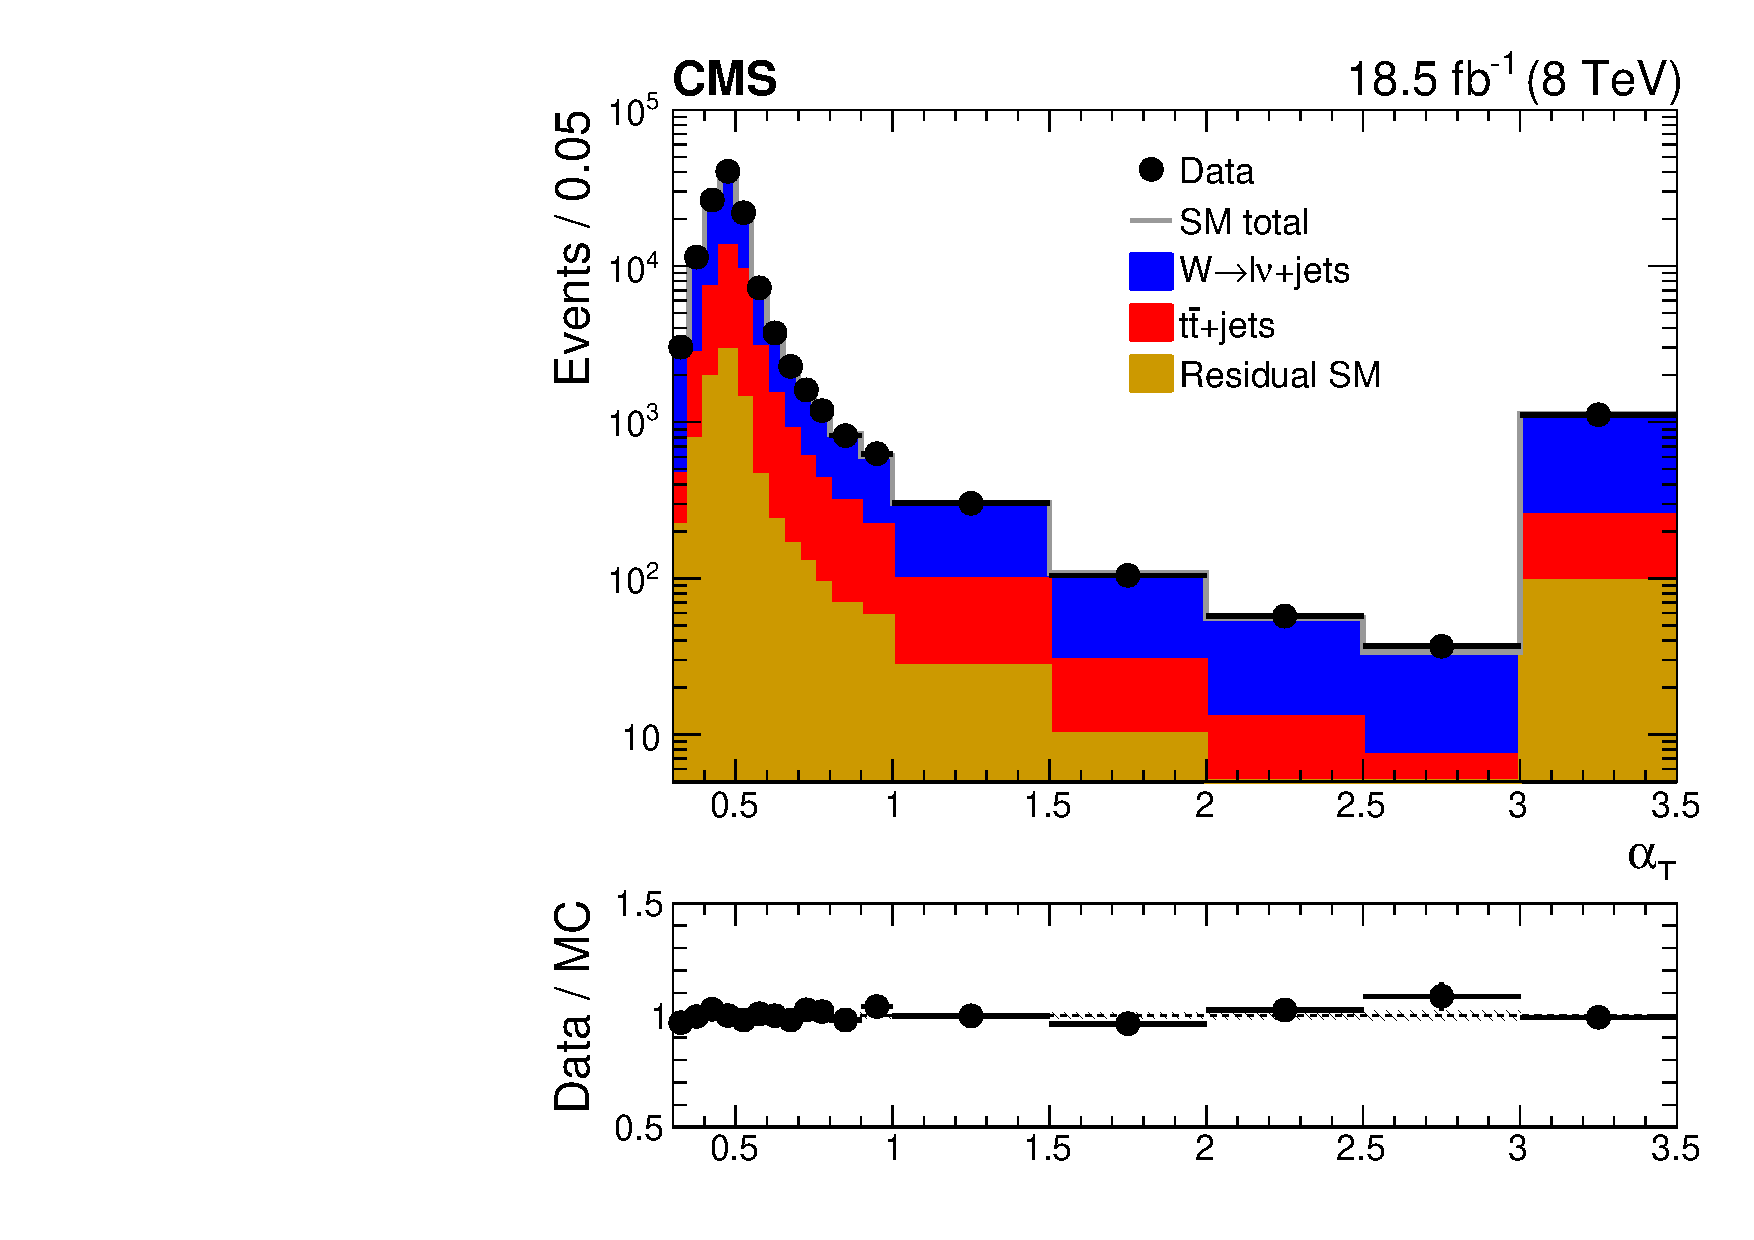
\includegraphics[width=0.48\textwidth]{Figure_002-a.pdf} ~~
  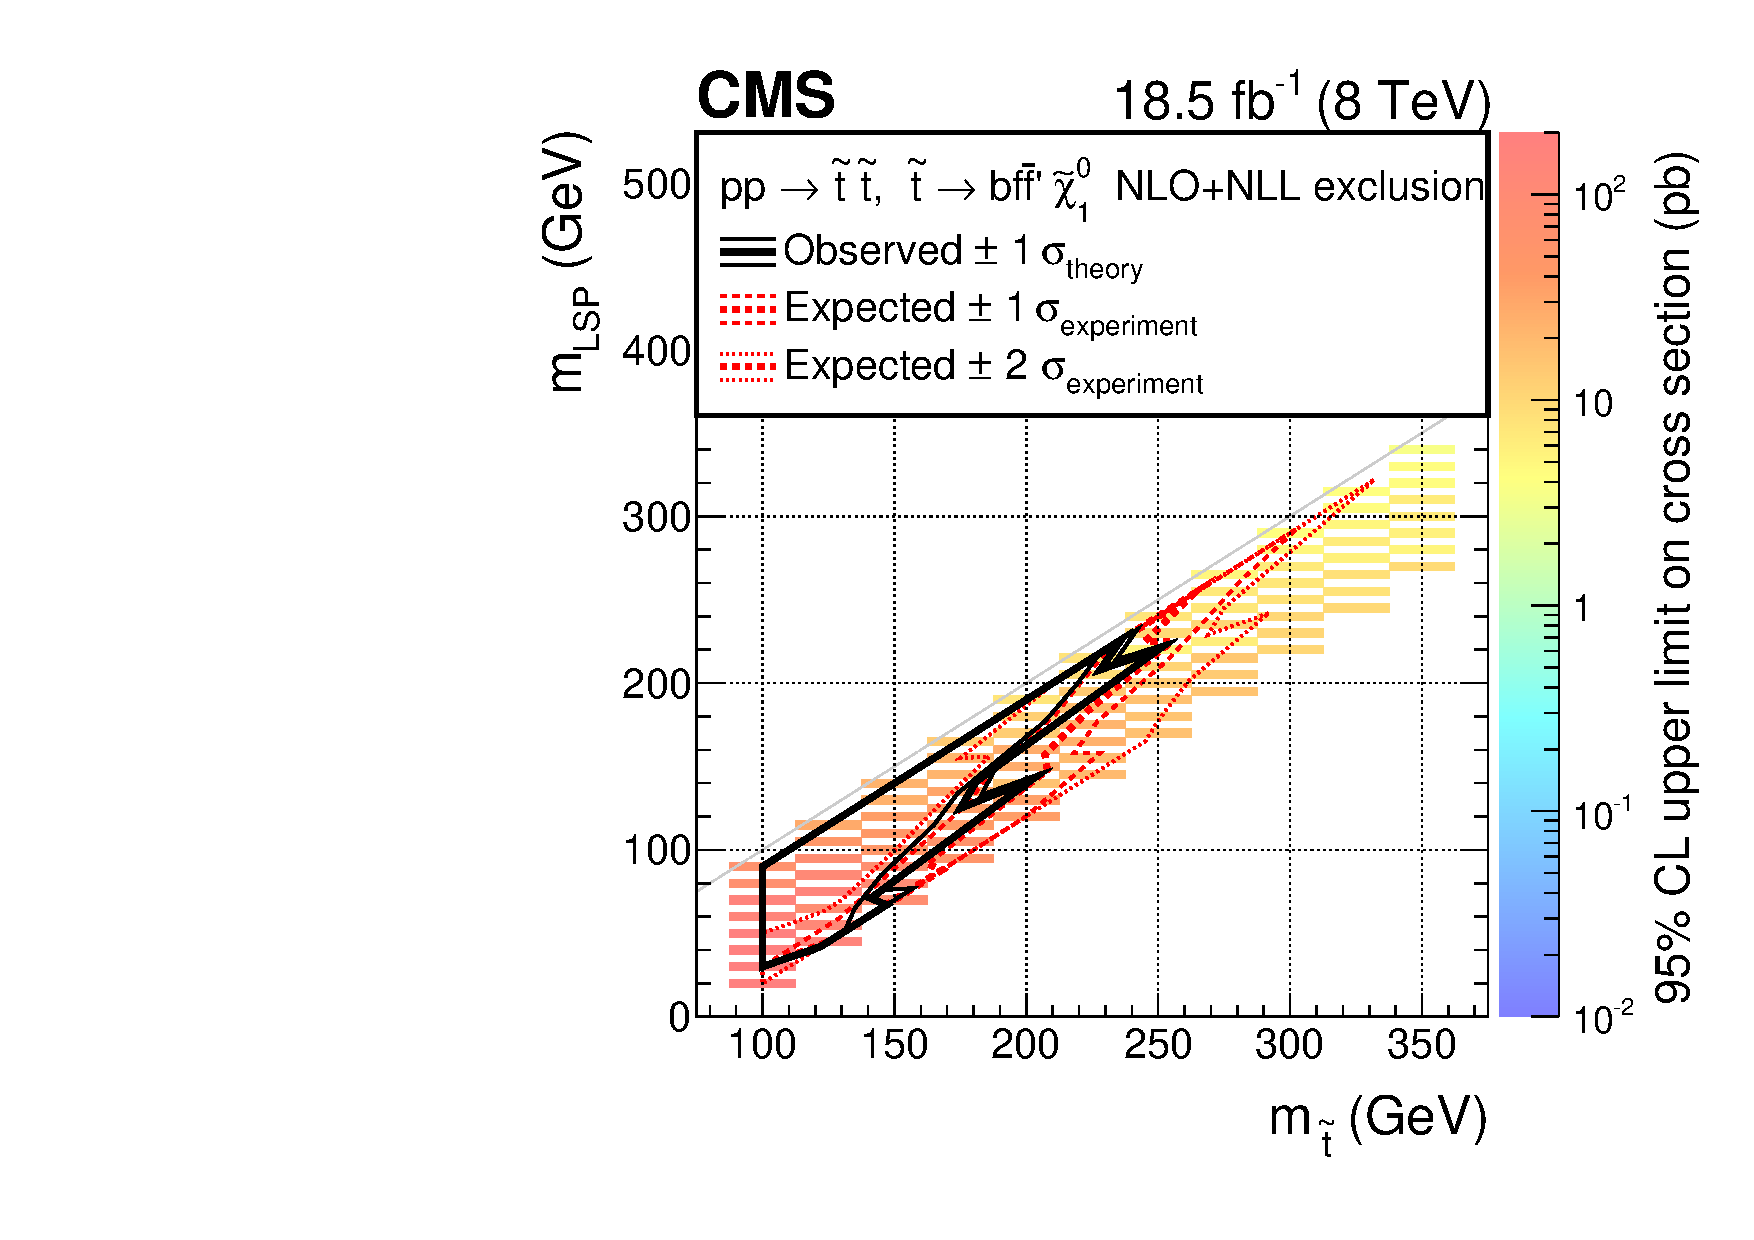
\includegraphics[width=0.48\textwidth]{Figure_002-b.pdf}
  \caption{The \alphat distribution observed in data for event samples
    that are recorded with an inclusive set of trigger conditions and
    satisfy (left) the selection criteria that define the \mj control
    region or (right) the criteria that define the signal region, with
    the additional requirement $\scalht > 375\GeV$. Event yields
    observed in data (solid circles) and SM expectations determined
    from simulation (solid histograms) are shown. Contributions from
    single top quark, diboson, Drell-Yan, and \ttbar + gauge boson
    production are collectively labelled ``Residual SM''. The final
    bin contains the overflow events. The lower panels show the ratios
    of the binned yields obtained from data and Monte Carlo (MC)
    simulation as a function of $\alpha_\text{T}$. The statistical
    uncertainties in the SM expectations are represented by the
    hatched areas. \label{fig:alphat}
  }
\end{figure}

Figure~\ref{fig:alphat} shows the distributions of the \alphat
variable obtained from samples of events that satisfy the selection
criteria used to define the \mj control and signal regions, which
highlight the background composition of the two samples as determined
from simulation. While the figure also demonstrates an adequate
modelling of the \alphat variable with simulated events, the method
employed by the search to estimate the nonmultijet backgrounds is
designed to mitigate the effects of simulation mismodelling. 

The method relies on the use of transfer factors that are constructed
per bin (in terms of \njet, \nb, and \scalht) for each control sample
in data. The transfer factors are determined using simulated events,
and are given by the ratios of the expected yields in the
corresponding bins of the signal region and control samples. The
transfer factors are used to extrapolate from the event yield measured
in a data control sample to the expectation for background from a
particular SM process or processes in the signal region. The method
aims to minimise the effects of simulation mismodelling, as many
systematic biases are expected to largely cancel in the ratios used to
define the transfer factors. Uncertainties in the transfer factors are
determined from a data-derived approach, described below.

The \mj data sample provides an estimate of the total contribution
from \ttbar and W boson production, as well as of the residual
contributions from single top quark, diboson, and Drell--Yan
($\PQq\PAQq \to \PZ/\gamma^* \to \ell^+\ell^-$) production. Two
independent estimates of the background from \znunujets events with
$\nb \leq 1$ are determined, one from the \gj data sample and the
other from the \mmj data sample, which are considered simultaneously
in the likelihood function described in Section~\ref{sec:results}. The
\gj and \zmumujets processes have similar kinematic properties when
the photon or muons are ignored in the determination of \ETmiss and
\HTmiss~\cite{Bern:2011pa}, although the acceptances differ. An
advantage of the \gj process is its much larger production cross
section compared to the \znunujets process. In the case of events with
$\nb \geq 2$, the \mj sample is also used to estimate the small
\znunujets background because of the limited event counts in the \mmj
and \gj control samples. Hence, only the \mj sample is used to
estimate the total SM background for events with $\nb \geq 2$, whereas
all three data control samples are used for events with $\nb \leq 1$.

To maximise sensitivity to new-physics signatures with a large number
of b quarks, a method is employed that improves the statistical
precision of the predictions from simulation, particularly for
$N_\cPqb \ge 2$~\cite{RA1Paper2012}. The distribution of $N_\cPqb$ is
estimated from generator-level information contained in the
simulation, namely the number of reconstruction-level jets matched to
underlying b quarks ($N_\cPqb^\text{gen}$), c quarks
($N_\cPqc^\text{gen}$), and light-flavoured quarks and gluons
($N_\cPq^\text{gen}$) per event. All relevant combinations of
$N_\cPqb^\text{gen}$, $N_\cPqc^\text{gen}$, and $N_{\cPq}^\text{gen}$
are considered, and events are categorised in terms of \njet and
\scalht.  The efficiency $\epsilon$ with which b quark jets are
identified, and the misidentification probabilities for c quarks and
light-flavour partons, $f_\cPqc$ and $f_\cPq$, respectively, are
determined from simulation for each event category, with each quantity
averaged over jet \pt and $\eta$. Corrections to $\epsilon$,
$f_\cPqc$, and $f_\cPq$ are applied on a jet-by-jet basis as a
function of \pt and $\eta$ so that they match the corresponding
quantity measured in data~\cite{Chatrchyan:2012jua}. This information
is sufficient to predict $N_\cPqb$ and determine the event yield from
simulation for a given event category. The event yields for a given b
quark jet multiplicity can be predicted with a higher statistical
precision than obtained directly from simulation, particularly for
events with a large number of b quark jets. These event yields are
subsequently used to determine the transfer factors binned according
to \nb (in addition to \njet and \scalht).

The uncertainties in the transfer factors obtained from simulation are
evaluated through sets of closure tests based events from the data
control regions~\cite{RA1Paper2012}. Each set uses the observed event
counts in up to eleven bins in \scalht for a given sample of events,
along with the corresponding (\scalht-dependent) transfer factors
obtained from simulation, to determine \scalht-dependent predictions
$N_\text{pred}(\scalht)$ for yields in another event sample. The two
samples are taken from different data control regions, or are subsets
of the same data control sample with differing requirements on \njet
or \nb. The predictions $N_\text{pred}(\scalht)$ are compared with the
\scalht-binned observed yields $N_\text{obs}(\scalht)$ and the level
of closure is defined by the deviation of the ratio $(N_\text{obs} -
N_\text{pred})/N_\text{pred}$ from zero. A large number of tests are
performed to probe key aspects of the modelling that may introduce an
\njet- or \scalht-dependent source of bias in the transfer
factors~\cite{RA1Paper2012}.

\begin{figure}[htbp]
  \centering
      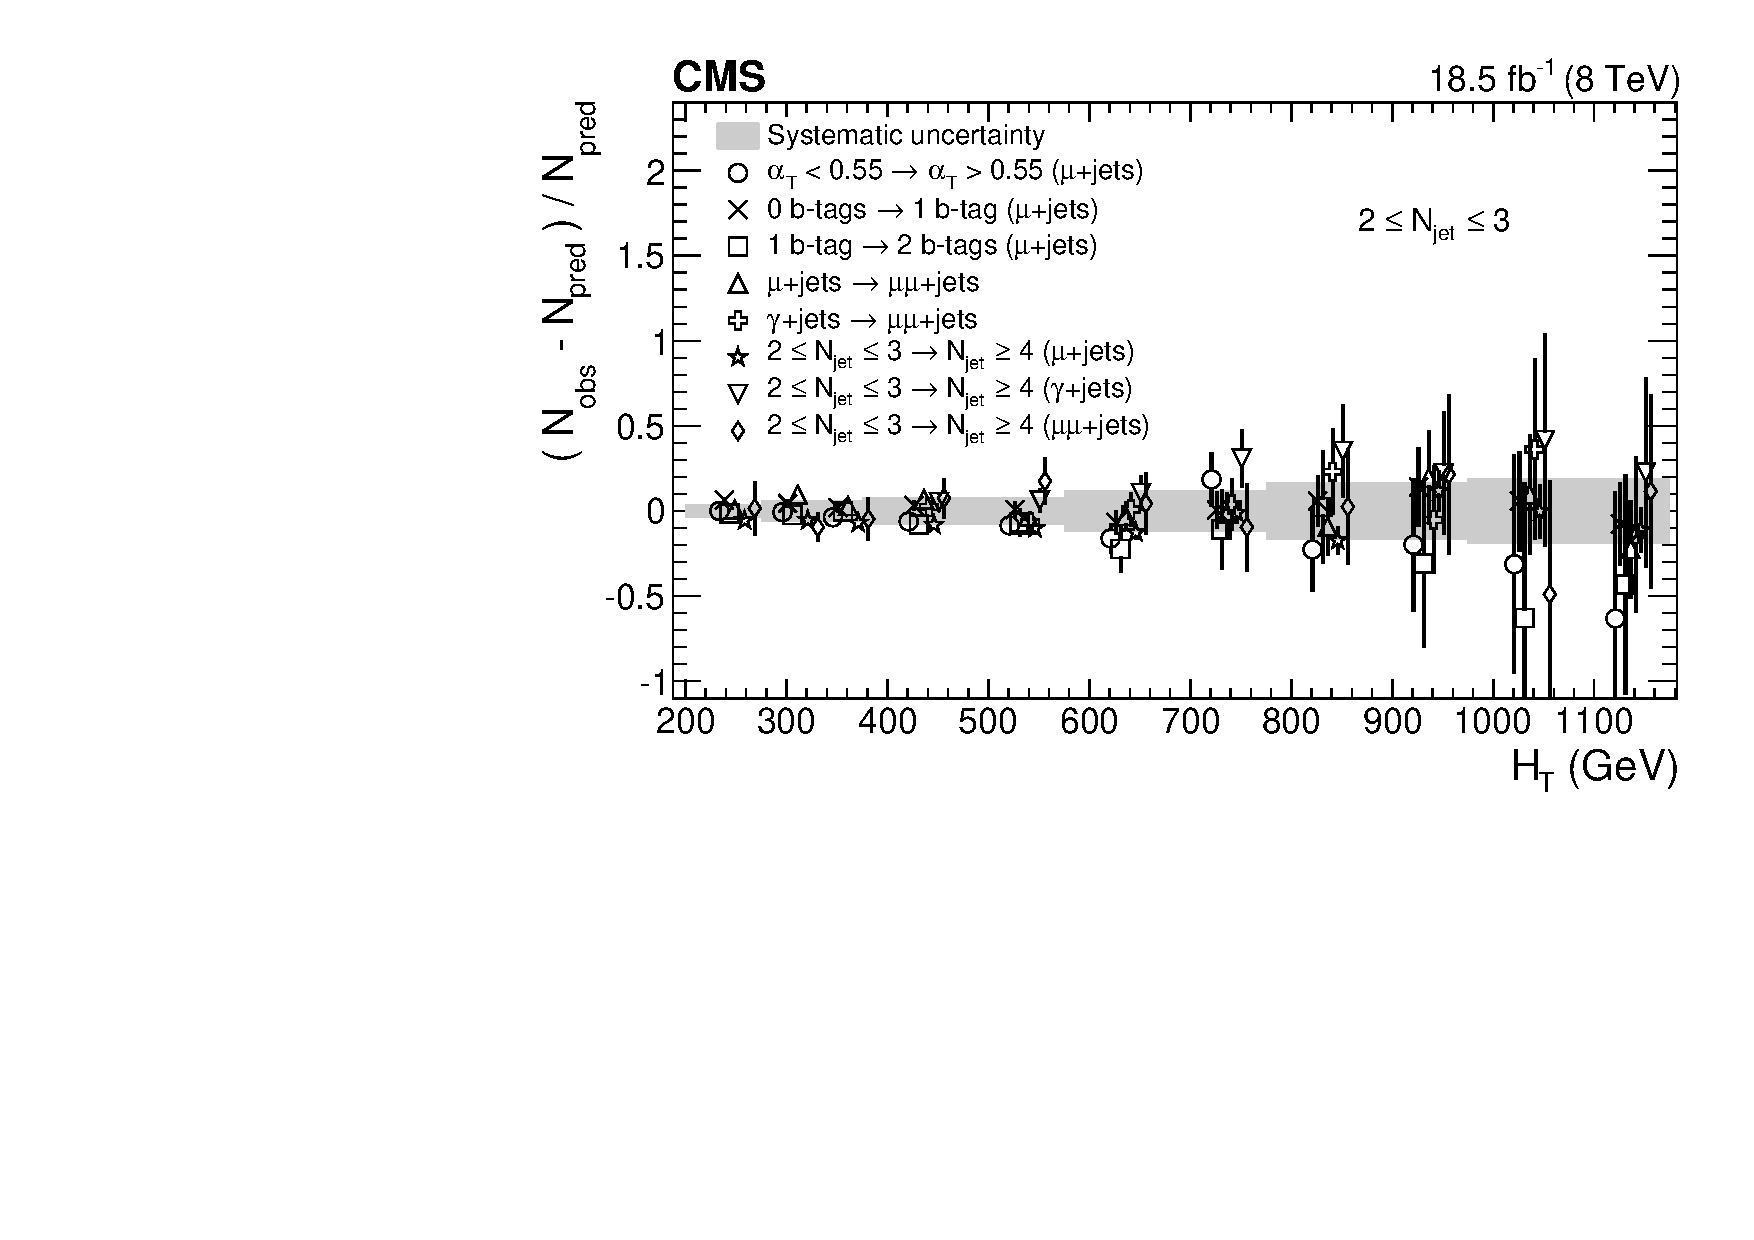
\includegraphics[width=\cmsFigWidth]{Figure_001-a.pdf}
      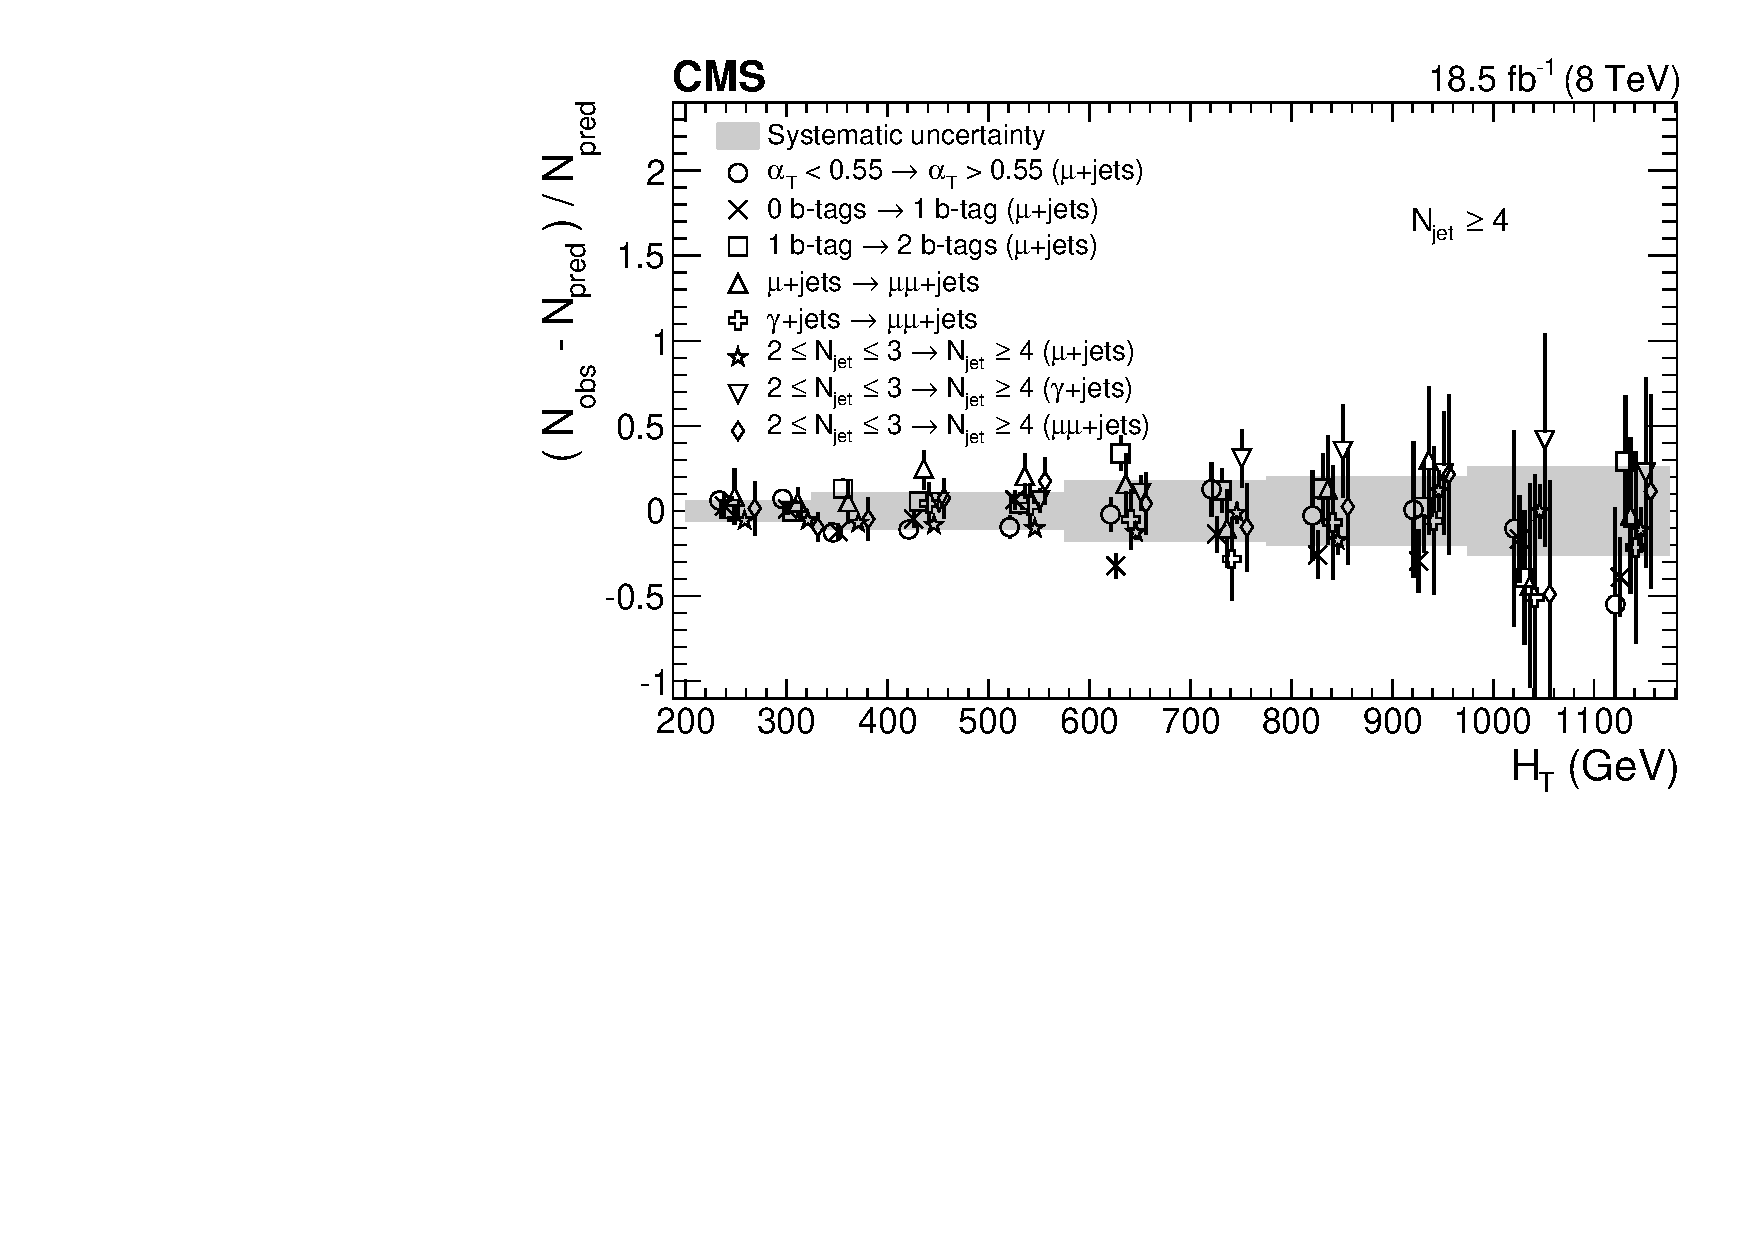
\includegraphics[width=\cmsFigWidth]{Figure_001-b.pdf}
    \caption{
      Ratio $(N_\text{obs} - N_\text{pred})/N_\text{pred}$ as a
      function of \scalht for different event categories and/or
      control regions for (upper) events with two or three jets, and
      (lower) events with four or more jets; ``b tag'' refers to a
      reconstructed b quark candidate.
      Error bars represent statistical uncertainties only, while the
      grey shaded bands represent the \njet- and \scalht-dependent
      uncertainties assumed in the transfer factors, as determined
      from the procedure described in the text.
      \label{fig:closure}
    }
\end{figure}

Systematic uncertainties are determined from core sets of closure
tests, of which the results are shown in Fig.~\ref{fig:closure}. Five
sets of tests are performed independently for each of the two \njet
categories, and a further three sets that are common to both \njet
categories. The tests aim to probe for the presence of statistically
significant biases that could arise due to limitations in the
method. For each \njet category, the first three sets of closure tests
are performed using the \mj sample. The first set probes the modelling
of the \alphat distribution for events containing genuine \ptvecmiss
from neutrinos (open circle markers). Two sets (crosses, squares)
probe the relative composition between \wjets and top events and the
modelling of the reconstruction of b quark jets. The fourth set
(triangles) validates the modelling of vector boson production by
connecting the \mj and \mmj control samples, which are enriched in
\wjets and \zjets events, respectively. The fifth set (swiss crosses)
deals with the consistency between the \gj and \mmj samples, which are
both used to provide an estimate of the \znunujets background. Three
further sets of closure tests (stars, inverted triangles, diamonds),
one per data control sample, probe the simulation modelling of the
\njet distribution for a range of background compositions.

\begin{table*}[!t]
  \topcaption{Systematic uncertainties (\%) in the transfer factors,
    in intervals of \njet and \scalht.}
  \label{tab:syst-values}
  \centering
  \begin{tabular}{ l*{7}r }
    \hline
            & \multicolumn{7}{c}{\scalht region (\GeVns)}                                \\
    \cline{2-8}
    \njet   & \multicolumn{1}{c}{200--275} & \multicolumn{1}{c}{275--325} & \multicolumn{1}{c}{325--375} & \multicolumn{1}{c}{375--575} & \multicolumn{1}{c}{575--775} & \multicolumn{1}{c}{775-975} & \multicolumn{1}{c}{$>975$} \\
    \hline
    2--3    & 4        & 6        & 6        & 8        & 12       & 17      & 19     \\
    $\geq4$ & 6        & 6        & 11       & 11       & 18       & 20      & 26     \\
    \hline
  \end{tabular}
\end{table*}

The closure tests reveal no significant biases or dependency on \njet
nor \scalht. Systematic uncertainties in the transfer factors are
determined from the variance in $(N_\text{obs} -
N_\text{pred})/N_\text{pred}$, weighted to account for statistical
uncertainties, for all closure tests within an individual \scalht bin
in the range $200 < \scalht < 375\GeV$ and for each \njet
category. For the region $\scalht > 375\GeV$, all tests within
200\GeV-wide intervals in \scalht, defined by pairs of adjacent bins,
are combined to determine the systematic uncertainty, which is assumed
to be fully correlated for bins within each interval, and fully
uncorrelated for different \scalht intervals and \njet categories. The
magnitudes of the systematic uncertainties are indicated by shaded
grey bands in Fig.~\ref{fig:closure} and summarised in
Table~\ref{tab:syst-values}. The same (uncorrelated) value of
systematic uncertainty is assumed for each \nb category. An
independent study is performed to assess the effect of uncertainties
in the simulation modelling of the efficiency and misidentification
rates for jets originating from b quarks and from light-flavoured
quarks or gluons. These uncertainties are found to be at the
sub-percent level, subdominant relative to the values in
Table~\ref{tab:syst-values}, and therefore considered to be
negligible.

\section{Results and interpretation\label{sec:results}}

For a given category of events satisfying requirements on both \njet
and \nb, a likelihood model of the observations in all data samples is
used to obtain a consistent prediction of the SM backgrounds and to
test for the presence of a variety of signal models. This is written
as:

\begin{equation}
  \label{likelihood}
  \begin{aligned}
  L_{\njet,\,\nb}  & =  L_\mathrm{SR} L_{\mu} L_{\mu\mu} L_{\gamma}, & (0 \leq \nb \leq 1) \\
  L_{\njet,\,\nb}  & =  L_\mathrm{SR} L_{\mu}, & (\nb \geq 2)
  \end{aligned}
\end{equation}

where $L_\mathrm{SR}$ is a likelihood function that describes the
yields in each of the \scalht bins of the signal region for given
values of \njet and \nb.  In each bin of \scalht, the observation is
modelled as a Poisson variable distributed about the sum of the SM
expectation and a potential contribution from a signal model (assumed
to be zero in the following discussion). The contribution from
multijet production is assumed to be zero, based on the studies
described in Section~\ref{sec:multijet}.  The SM expectation in the
signal region is related to the expected yields in the \mj, \mmj, and
\gj control samples via the transfer factors derived from
simulation. The likelihood functions $L_\mu$, $L_{\mu\mu}$, and
$L_\gamma$ describe the yields in the \scalht bins of the \mj, \mmj,
and \gj control samples for the same values of \njet and \nb as the
signal region.  For the category of events with $\nb \geq 2$, only the
\mj control sample is used in the likelihood to determine the total
contribution from all nonmultijet SM backgrounds in the signal
region. The systematic uncertainties in the transfer factors,
determined from the ensemble of closure tests described above and with
magnitudes in the range 4--26\% (Table~\ref{tab:syst-values}), are
accommodated in the likelihood function through a nuisance parameter
per (\njet, \nb) category per \scalht interval per transfer
factor. The measurements of these parameters are assumed to follow a
lognormal distribution.

\begin{table*}[!t]
  \topcaption{
    Observed event yields in data and the ``a priori'' SM expectations
    determined from event counts in the data control samples and
    transfer factors from simulation, in bins of \scalht, and
    categorised according to \njet and \nb. Also shown are the SM
    expectations (labelled ``SM'') obtained from a combined fit to
    control and signal regions under the SM hypothesis. The quoted
    uncertainties include the statistical as well as systematic
    components. For each row that lists fewer than the full set of
    columns, the final entry represents values obtained for an open
    final \scalht bin. 
  }
  \label{tab:fit-result}
  \centering
  \resizebox{\textwidth}{!}{
  \renewcommand*{\arraystretch}{1.4}
  \begin{tabular}{ lllllllllllll }
    \hline
    Category &  & \multicolumn{11}{c}{\scalht (\GeVns)} \\
    \cline{3-13}
    (\njet,\,\nb)
             & 
             & 200--275
             & 275--325
             & 325--375
             & 375--475
             & 475--575
             & 575--675
             & 675--775
             & 775--875
             & 875--975
             & 975--1075
             & 1075--$\infty$                           \\
    \hline
    (2--3,\,0)
             & Data
             & $13090$
             & $5331$
             & $3354$
             & $2326$
             & $671$
             & $206$
             & $76$
             & $29$
             & $10$
             & $9$
             & $2$                                      \\
    (2--3,\,0)
             & a priori
             & $12410^{+370}_{-410}$
             & $5540^{+340}_{-230}$
             & $3330^{+130}_{-170}$
             & $2400^{+120}_{-90}$
             & $663^{+34}_{-26}$
             & $225^{+21}_{-17}$
             & $68.5^{+6.9}_{-6.7}$
             & $26.5^{+3.9}_{-3.0}$
             & $10.3^{+1.9}_{-2.1}$
             & $5.1^{+1.0}_{-1.1}$
             & $4.5^{+0.9}_{-0.9}$                      \\
    (2--3,\,0)
             & SM
             & $13030^{+90}_{-120}$
             & $5348^{+85}_{-67}$
             & $3351^{+56}_{-50}$
             & $2351^{+38}_{-45}$
             & $655^{+14}_{-11}$
             & $218^{+12}_{-17}$
             & $68.5^{+4.9}_{-4.8}$
             & $27.2^{+3.0}_{-3.0}$
             & $10.4^{+1.5}_{-1.6}$
             & $5.6^{+1.0}_{-1.0}$
             & $4.3^{+0.7}_{-1.0}$                      \\\\[-2ex]
    (2--3,\,1)
             & Data
             & $1733$
             & $833$
             & $527$
             & $356$
             & $90$
             & $31$
             & $6$
             & $4$
             & $1$
             & $0$
             & $1$                                      \\
    (2--3,\,1)
             & a priori
             & $1669^{+65}_{-67}$
             & $853^{+50}_{-46}$
             & $525^{+37}_{-24}$
             & $391^{+23}_{-21}$
             & $94.3^{+6.0}_{-5.6}$
             & $24.5^{+2.5}_{-3.6}$
             & $9.0^{+1.2}_{-1.4}$
             & $2.8^{+0.6}_{-0.8}$
             & $2.5^{+0.8}_{-0.9}$
             & $0.3^{+0.2}_{-0.1}$
             & $0.2^{+0.1}_{-0.1}$                      \\
    (2--3,\,1)
             & SM
             & $1711^{+37}_{-33}$
             & $839^{+21}_{-25}$
             & $526^{+20}_{-17}$
             & $372^{+12}_{-14}$
             & $90.6^{+5.1}_{-4.6}$
             & $25.8^{+2.9}_{-2.6}$
             & $8.7^{+0.8}_{-1.4}$
             & $3.0^{+0.7}_{-0.6}$
             & $2.2^{+0.8}_{-0.6}$
             & $0.3^{+0.2}_{-0.1}$
             & $0.2^{+0.1}_{-0.2}$                      \\\\[-2ex]
    (2--3,\,2)
             & Data
             & $172$
             & $116$
             & $101$
             & $55$
             & $16$
             & $9$
             & $0$
             & $0$
             & $0$                                      \\
    (2--3,\,2)
             & a priori
             & $187^{+7}_{-8}$
             & $118^{+7}_{-7}$
             & $98.7^{+7.1}_{-7.0}$
             & $61.3^{+5.9}_{-5.5}$
             & $12.3^{+1.7}_{-1.0}$
             & $2.8^{+0.5}_{-0.6}$
             & $0.7^{+0.2}_{-0.2}$
             & $0.2^{+0.1}_{-0.1}$
             & $<$0.1                                   \\
    (2--3,\,2)
             & SM
             & $184^{+5}_{-7}$
             & $117^{+7}_{-5}$
             & $99.4^{+5.4}_{-4.6}$
             & $60.2^{+3.5}_{-3.8}$
             & $12.4^{+1.2}_{-1.0}$
             & $3.3^{+0.6}_{-0.5}$
             & $0.7^{+0.2}_{-0.2}$
             & $0.2^{+0.1}_{-0.1}$
             & $<$0.1                                   \\\\[-2ex]
    ($\geq4$,\,0)
             & Data
             & $99$
             & $568$
             & $408$
             & $336$
             & $211$
             & $117$
             & $38$
             & $13$
             & $9$
             & $4$
             & $6$                                      \\
    ($\geq4$,\,0)
             & a priori
             & $108^{+10}_{-12}$
             & $497^{+34}_{-36}$
             & $403^{+36}_{-33}$
             & $327^{+25}_{-22}$
             & $193^{+14}_{-13}$
             & $95^{+13}_{-11}$
             & $40.3^{+5.9}_{-4.4}$
             & $14.5^{+3.5}_{-2.4}$
             & $7.1^{+1.7}_{-1.4}$
             & $3.2^{+0.7}_{-1.0}$
             & $2.9^{+0.7}_{-0.5}$                      \\
    ($\geq4$,\,0)
             & SM
             & $104^{+6}_{-8}$
             & $544^{+21}_{-18}$
             & $407^{+18}_{-18}$
             & $337^{+15}_{-10}$
             & $202^{+10}_{-8}$
             & $105^{+9}_{-7}$
             & $42.5^{+4.5}_{-3.3}$
             & $14.3^{+1.7}_{-2.5}$
             & $7.5^{+1.4}_{-1.5}$
             & $3.5^{+0.8}_{-0.8}$
             & $3.4^{+1.0}_{-0.7}$                      \\\\[-2ex]
    ($\geq4$,\,1)
             & Data
             & $38$
             & $195$
             & $210$
             & $159$
             & $83$
             & $33$
             & $7$
             & $10$
             & $4$
             & $1$
             & $1$                                      \\
    ($\geq4$,\,1)
             & a priori
             & $39.2^{+3.0}_{-3.5}$
             & $215^{+12}_{-16}$
             & $208^{+24}_{-22}$
             & $150^{+15}_{-11}$
             & $75.8^{+7.8}_{-6.6}$
             & $28.6^{+3.8}_{-3.7}$
             & $10.3^{+2.1}_{-1.4}$
             & $5.1^{+1.3}_{-0.9}$
             & $2.0^{+0.7}_{-0.5}$
             & $0.8^{+0.4}_{-0.3}$
             & $0.9^{+0.6}_{-0.4}$                      \\
    ($\geq4$,\,1)
             & SM
             & $38.9^{+2.2}_{-3.7}$
             & $206^{+12}_{-10}$
             & $209^{+13}_{-10}$
             & $157^{+9}_{-9}$
             & $79.3^{+5.2}_{-4.7}$
             & $29.4^{+3.8}_{-2.2}$
             & $9.9^{+1.9}_{-1.3}$
             & $6.2^{+1.2}_{-1.1}$
             & $2.3^{+0.7}_{-0.7}$
             & $0.9^{+0.3}_{-0.3}$
             & $0.9^{+0.3}_{-0.4}$                      \\\\[-2ex]
    ($\geq4$,\,2)
             & Data
             & $16$
             & $81$
             & $88$
             & $64$
             & $43$
             & $14$
             & $5$
             & $1$
             & $1$                                      \\
    ($\geq4$,\,2)
             & a priori
             & $12.3^{+1.0}_{-1.0}$
             & $76.7^{+5.6}_{-5.2}$
             & $93^{+11}_{-9}$
             & $63.0^{+7.8}_{-5.7}$
             & $34.0^{+3.6}_{-3.4}$
             & $10.1^{+2.6}_{-1.8}$
             & $3.4^{+0.9}_{-0.6}$
             & $1.0^{+0.2}_{-0.2}$
             & $0.7^{+0.1}_{-0.2}$                      \\
    ($\geq4$,\,2)
             & SM
             & $12.5^{+1.0}_{-1.0}$
             & $77.8^{+4.7}_{-4.6}$
             & $90.2^{+9.0}_{-6.5}$
             & $66.1^{+4.6}_{-4.8}$
             & $36.3^{+3.4}_{-2.9}$
             & $11.4^{+1.8}_{-1.9}$
             & $3.9^{+0.8}_{-0.7}$
             & $1.0^{+0.2}_{-0.3}$
             & $0.7^{+0.1}_{-0.2}$                      \\\\[-2ex]
    ($\geq4$,\,3)
             & Data
             & $0$
             & $7$
             & $5$
             & $5$
             & $6$
             & $1$
             & $1$
             & $0$
             & $0$                                      \\
    ($\geq4$,\,3)
             & a priori
             & $1.1^{+0.2}_{-0.1}$
             & $8.2^{+0.6}_{-0.9}$
             & $11.1^{+2.0}_{-1.6}$
             & $7.4^{+1.1}_{-1.0}$
             & $4.0^{+0.5}_{-0.6}$
             & $1.1^{+0.3}_{-0.3}$
             & $0.4^{+0.2}_{-0.1}$
             & $0.1^{+0.1}_{-0.0}$
             & $<$0.1                                   \\
    ($\geq4$,\,3)
             & SM
             & $1.1^{+0.2}_{-0.2}$
             & $8.1^{+0.9}_{-0.9}$
             & $9.9^{+1.5}_{-1.3}$
             & $7.2^{+0.9}_{-0.7}$
             & $4.1^{+0.6}_{-0.6}$
             & $1.1^{+0.3}_{-0.3}$
             & $0.4^{+0.1}_{-0.1}$
             & $0.1^{+0.1}_{-0.0}$
             & $<$0.1                                   \\\\[-2ex]
    ($\geq4$,\,$\geq4$)
             & Data
             & $0$
             & $0$
             & $0$
             & $2$                                      \\
    ($\geq4$,\,$\geq4$)
             & a priori 
             & $<$0.1
             & $0.2^{+0.1}_{-0.1}$
             & $0.5^{+0.3}_{-0.3}$
             & $0.3^{+0.2}_{-0.2}$                      \\
    ($\geq4$,\,$\geq4$)
             & SM
             & $<$0.1
             & $0.1^{+0.1}_{-0.1}$
             & $0.4^{+0.2}_{-0.3}$
             & $0.4^{+0.2}_{-0.2}$                      \\

    \hline
  \end{tabular}
  }
\end{table*}

Table~\ref{tab:fit-result} summarises the observed event yields and
expected number of events from SM processes in the signal region as a
function of \njet, \nb, and \scalht. The ``a priori'' SM expectations
are determined from event counts in the data control samples and
transfer factors from simulation, and are therefore independent of the
signal region. No significant discrepancies are observed between the
``a priori'' SM expectations and the observed events yields. In
addition, Table~\ref{tab:fit-result} summarises the expected number of
events from SM processes (labelled ``SM'') determined from a
simultaneous fit to data in up to three control samples and the signal
region. The likelihood function is maximised over all fit parameters
under the SM-only hypothesis. The $p$-value probabilities for all
\njet and \nb categories are found to be uniformly distributed, with a
minimum value of 0.19.

The results of this search are interpreted in terms of limits on the
parent sparticle and LSP masses in the parameter space of simplified
models~\cite{Alwall:2008ag, Alwall:2008va, sms} that represent the
direct pair production of top squarks and the decay modes $\PSQt
\to\PQc\PSGczDo$, $\PSQt \to{\PQb \ffbp} \PSGczDo$, $\PSQt \to \PQb
\PSGcpmDo$ followed by $\PSGcpmDo \to \PW^\pm \PSGczDo$, and $\PSQt
\to \PQt \PSGczDo$. The \cls method~\cite{read,junk} is used to
determine upper limits at the 95\% confidence level (CL) on the
production cross section of a signal model, using the one-sided
(LHC-style) profile likelihood ratio as the test
statistic~\cite{higgs-comb}. The sampling distributions for the test
statistic are constructed from likelihoods based on generated
pseudo-experiments, using the respective maximum likelihood values of
nuisance parameters extracted under the SM background-only and signal
+ background hypotheses. The potential contributions of signal events
to each of the signal and control samples are considered, but the only
significant contribution occurs in the signal region and not the
control samples.

The event samples for the simplified models are generated with the LO
\MADGRAPH 5.1.1.0 generator, which considers up to two additional
partons in the matrix element calculation. Inclusive,
process-dependent, NLO calculations of SUSY production cross sections,
with next-to-leading-logarithmic (NLL) corrections, are obtained with
the program \PROSPINO 2.1~\cite{Beenakker:1996ch, PhysRevD.80.095004,
  PhysRevLett.102.111802, PhysRevD.80.095004, 1126-6708-2009-12-041,
  doi:10.1142/S0217751X11053560, susy-nlo-nll}. All events are
generated using the \textsc{CTEQ6L1} PDFs. As for SM processes, the
simulated events are generated with a nominal pileup distribution and
then reweighted to match the distribution observed in data. The
detector response is provided by the CMS fast simulation
package~\cite{fastsim}.

Experimental uncertainties in the expected signal yields are
considered. Contributions to the overall systematic uncertainty arise
from various sources such as the uncertainties from the choice of
PDFs, the jet energy scale, the modelling of the efficiency and
misidentification probability of b quark jets in simulation, the
integrated luminosity~\cite{lumi}, and various event selection
criteria. The magnitude of each contribution depends on the model, the
masses of the parent sparticle and LSP, and the event category under
consideration. Uncertainties in the jet energy scale are typically
dominant ($\sim$15\%) for models with mass splittings that satisfy
$\dm > m_\PQt$, where $m_\PQt$ is the top quark mass. The acceptance
for models with mass splittings satisfying $\dm < m_\PQt$ is due in
large part to ISR, the modelling of which contributes the dominant
systematic uncertainty for systems with a compressed mass spectrum. An
uncertainty of $\sim$20\% is determined by comparing the simulated and
measured \pt spectra of the system recoiling against the ISR jets in
\ttbar events, using the technique described in
Ref.~\cite{single-lepton-stop}. For the aforementioned simplified
models, the effect of uncertainties in the distribution of signal
events is generally small compared with the uncertainties in the
experimental acceptance. The total systematic uncertainty in the yield
of signal is found to be in the range 5--36\%, depending on \njet and
\nb, and is taken into account through a nuisance parameter that
follows a lognormal distribution.

\begin{figure*}[htbp]
\centering
      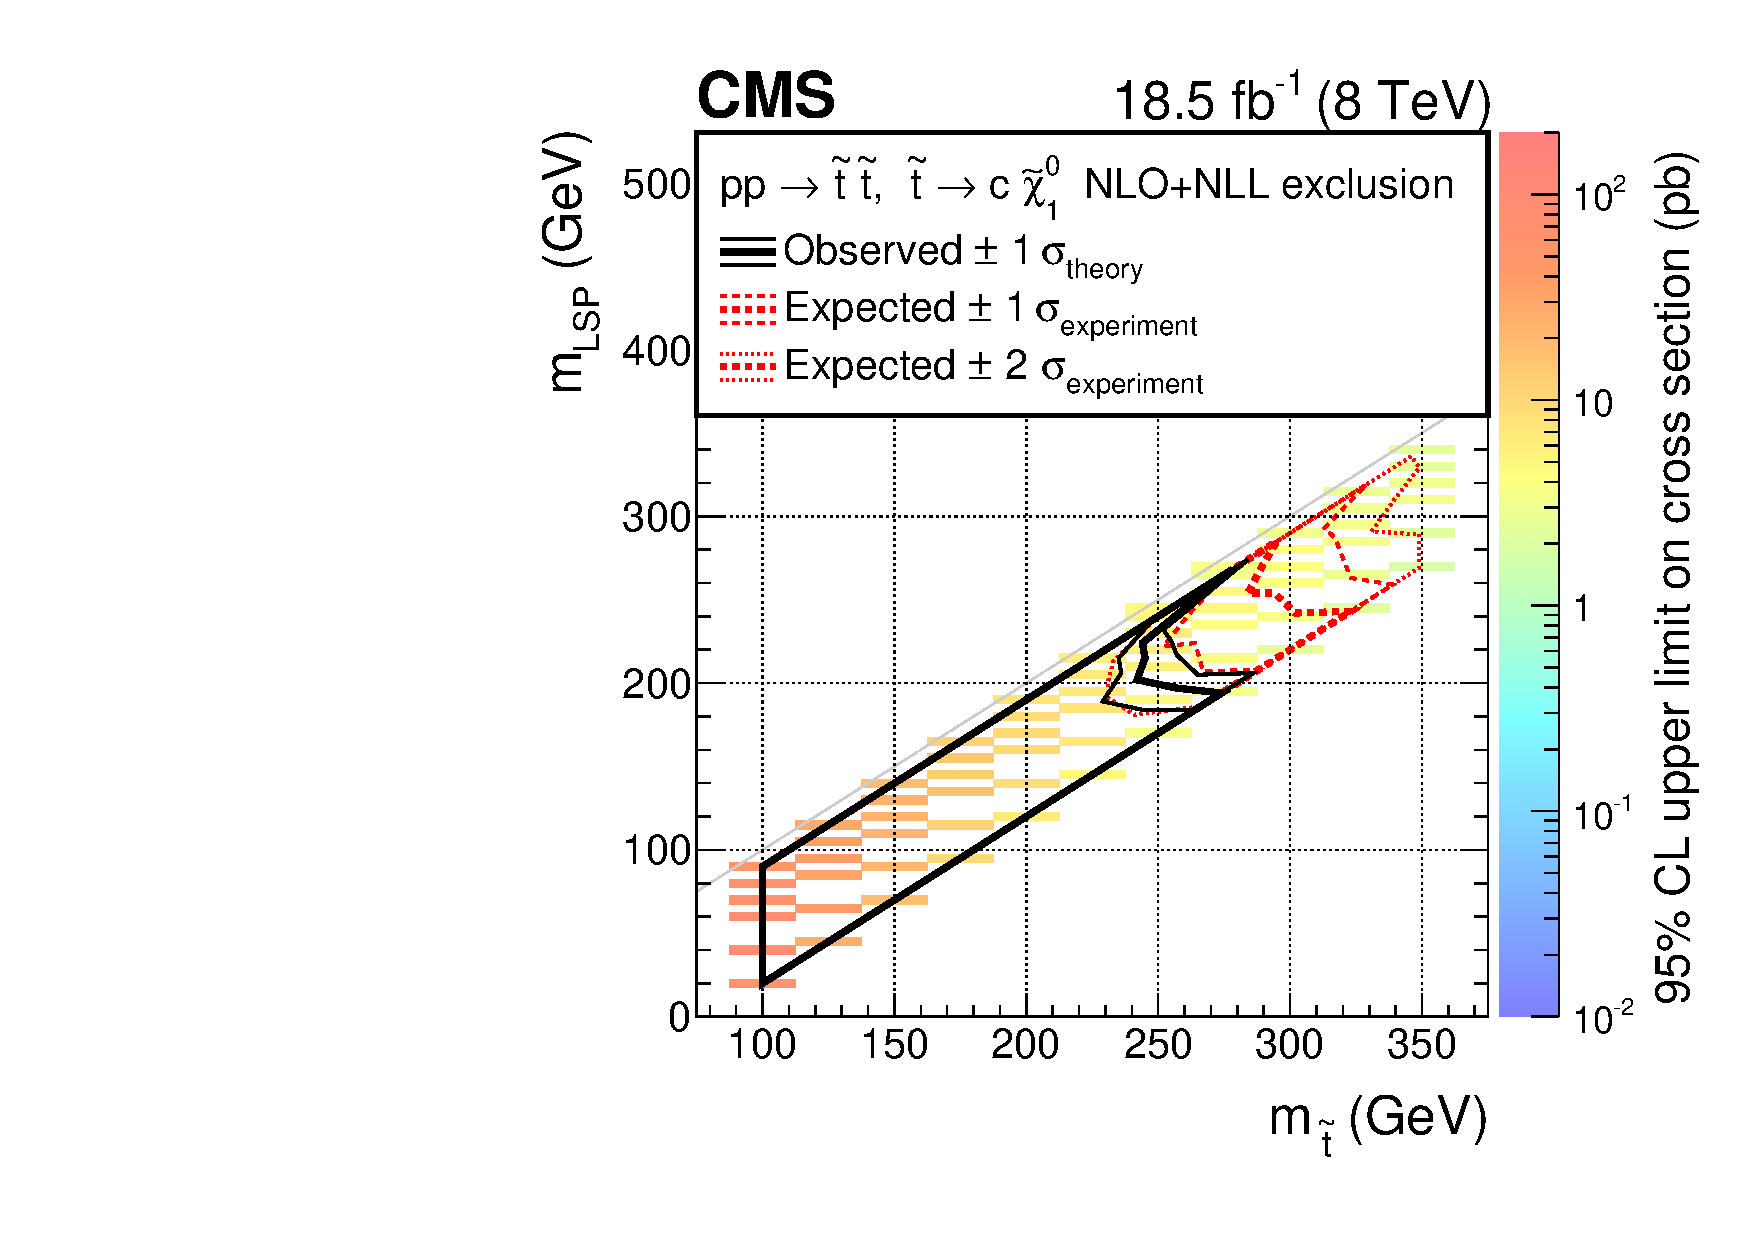
\includegraphics[width=0.40\textwidth]{Figure_003-a.pdf}
      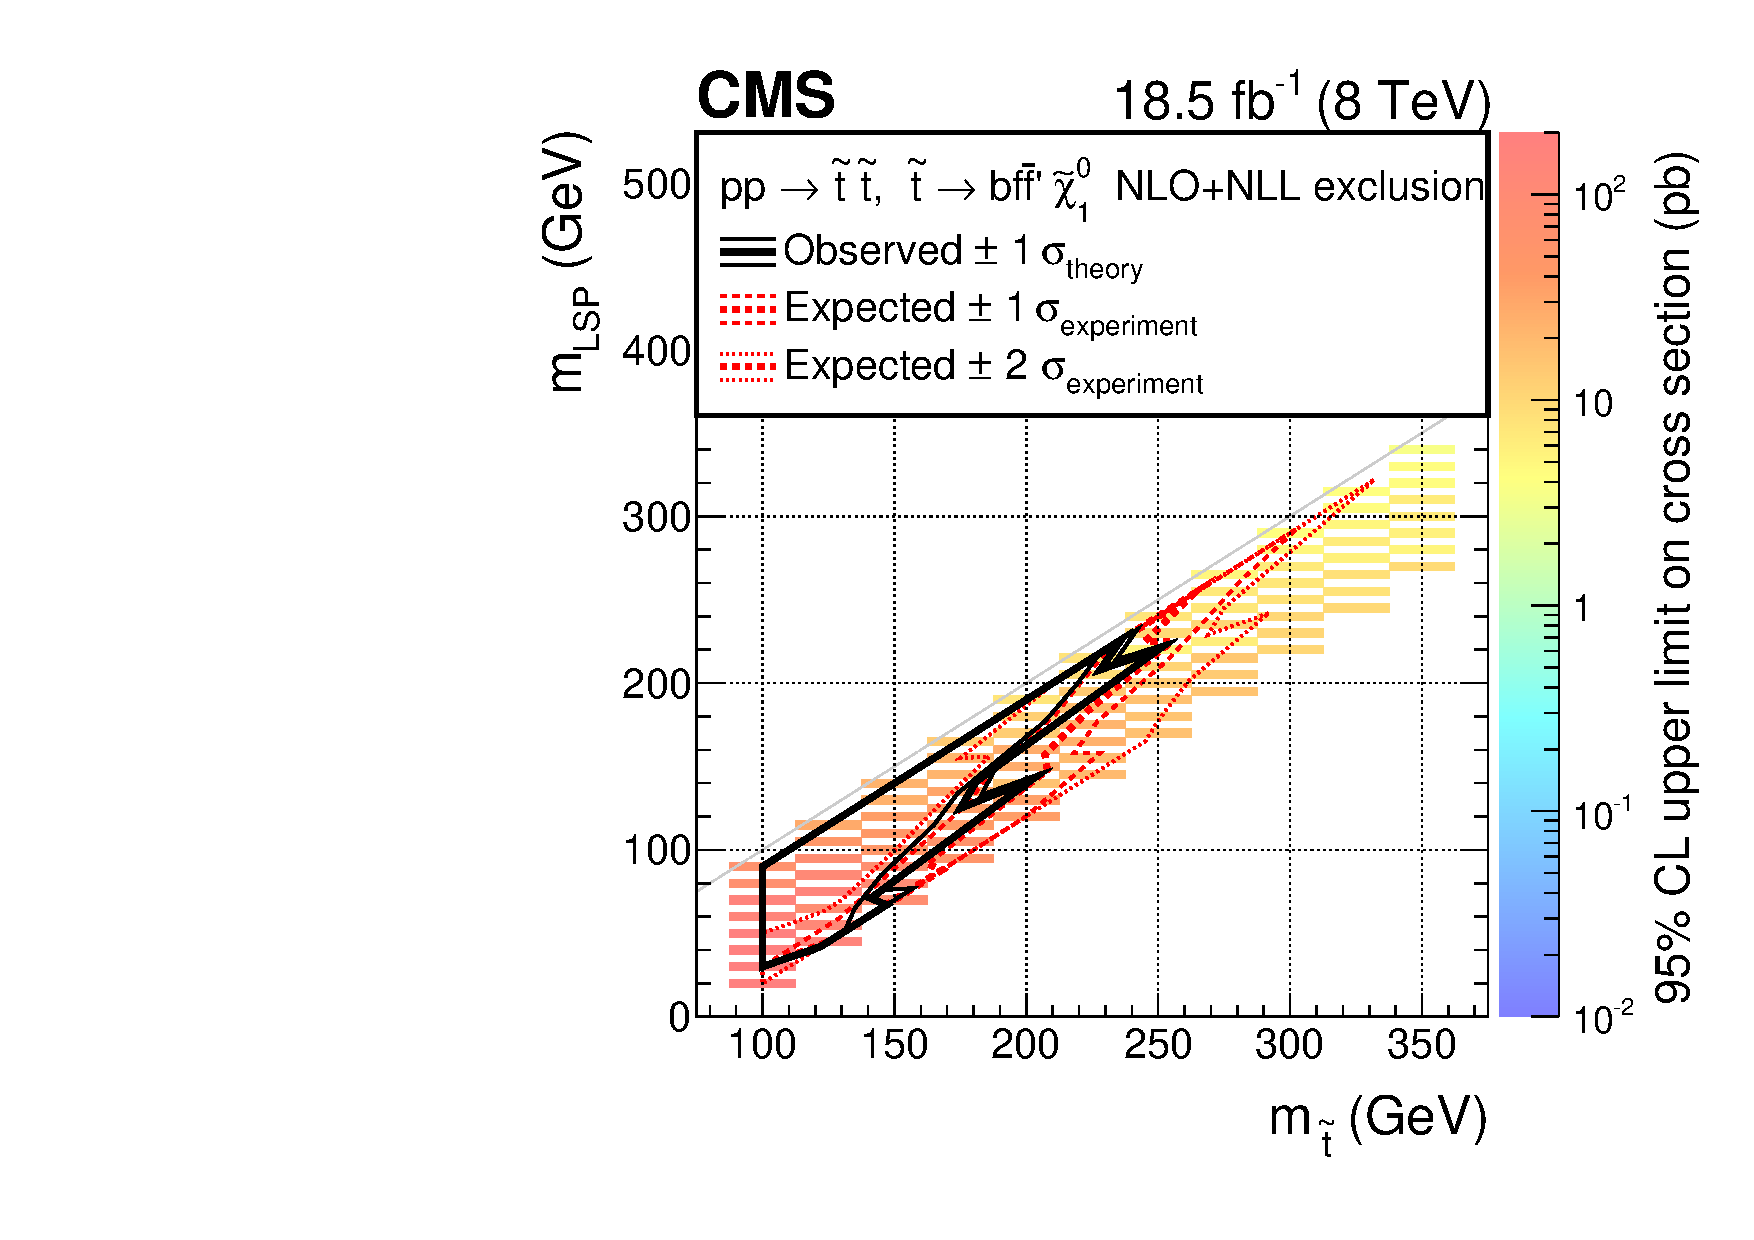
\includegraphics[width=0.40\textwidth]{Figure_003-b.pdf}
      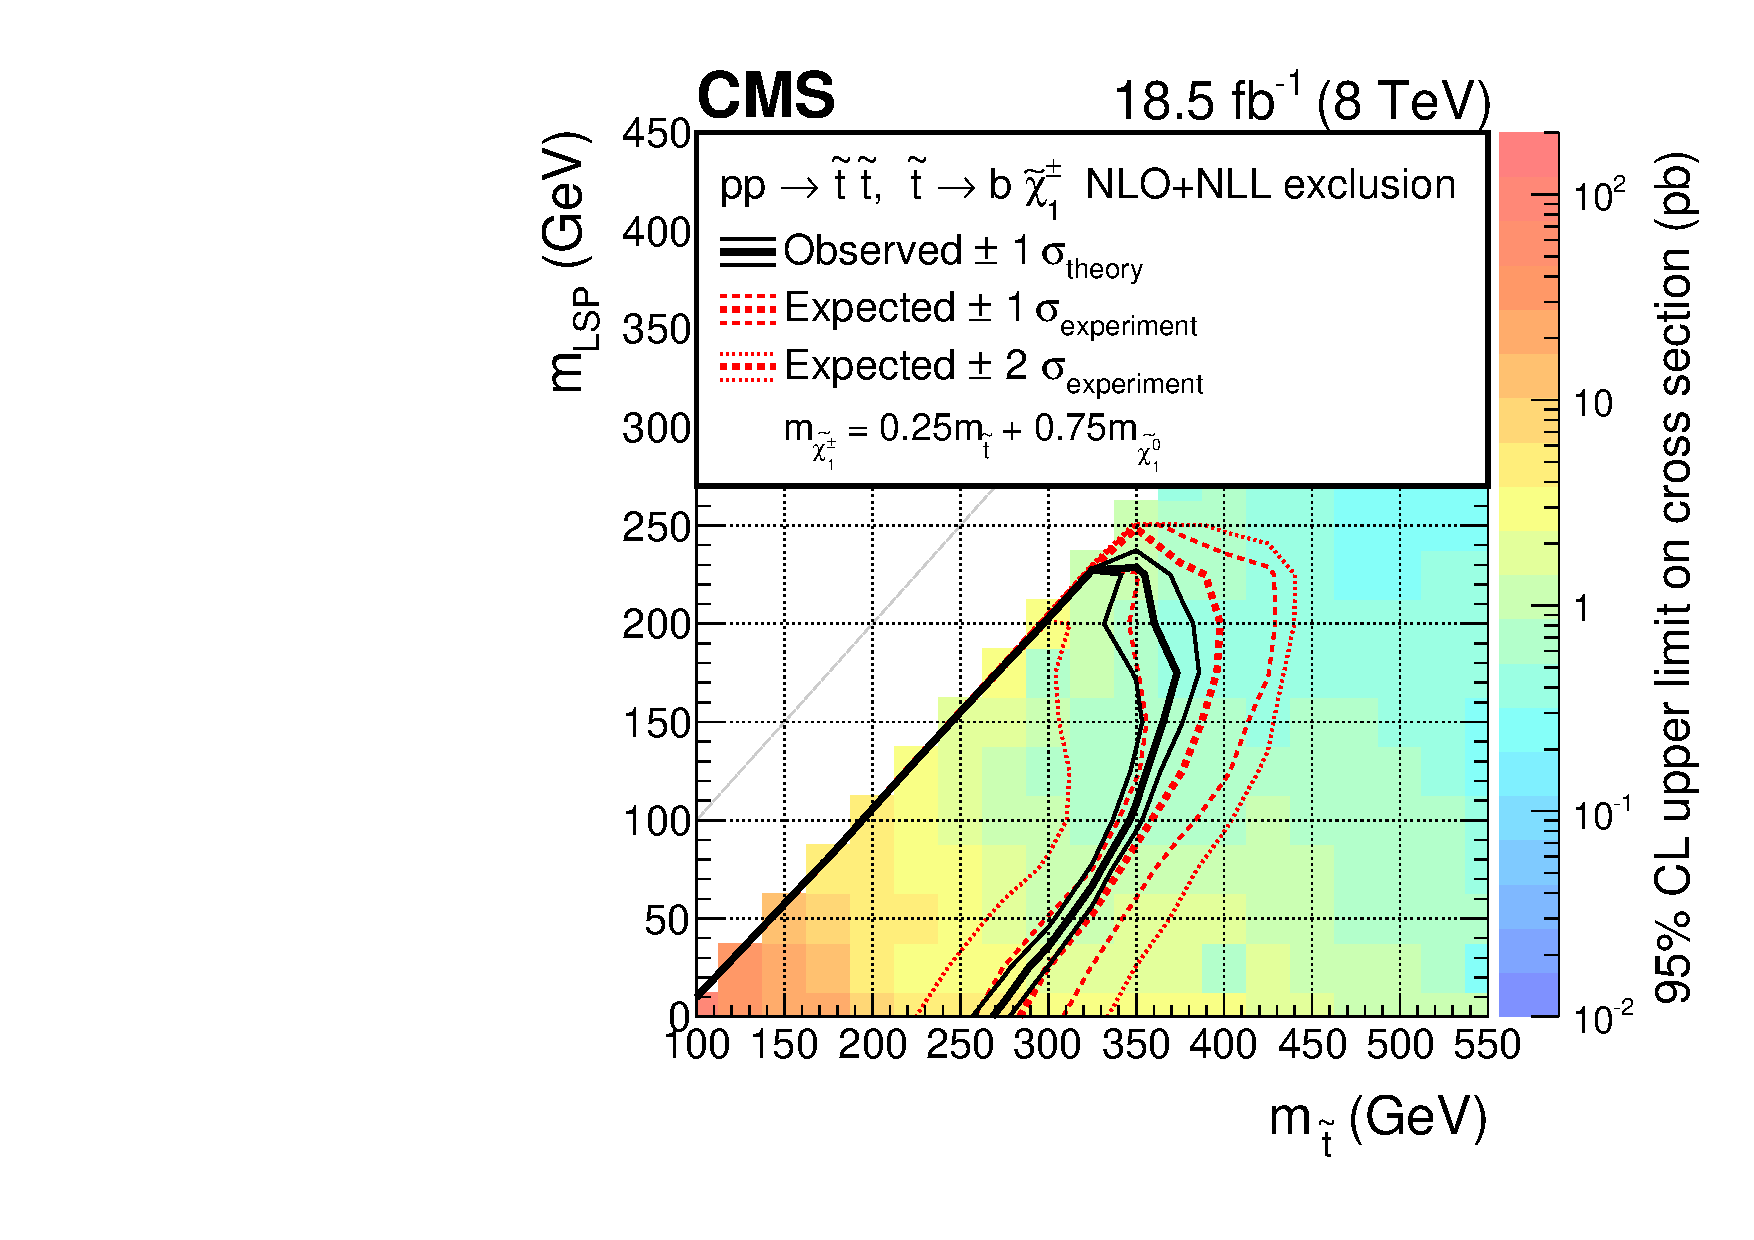
\includegraphics[width=0.40\textwidth]{Figure_003-c.pdf}
      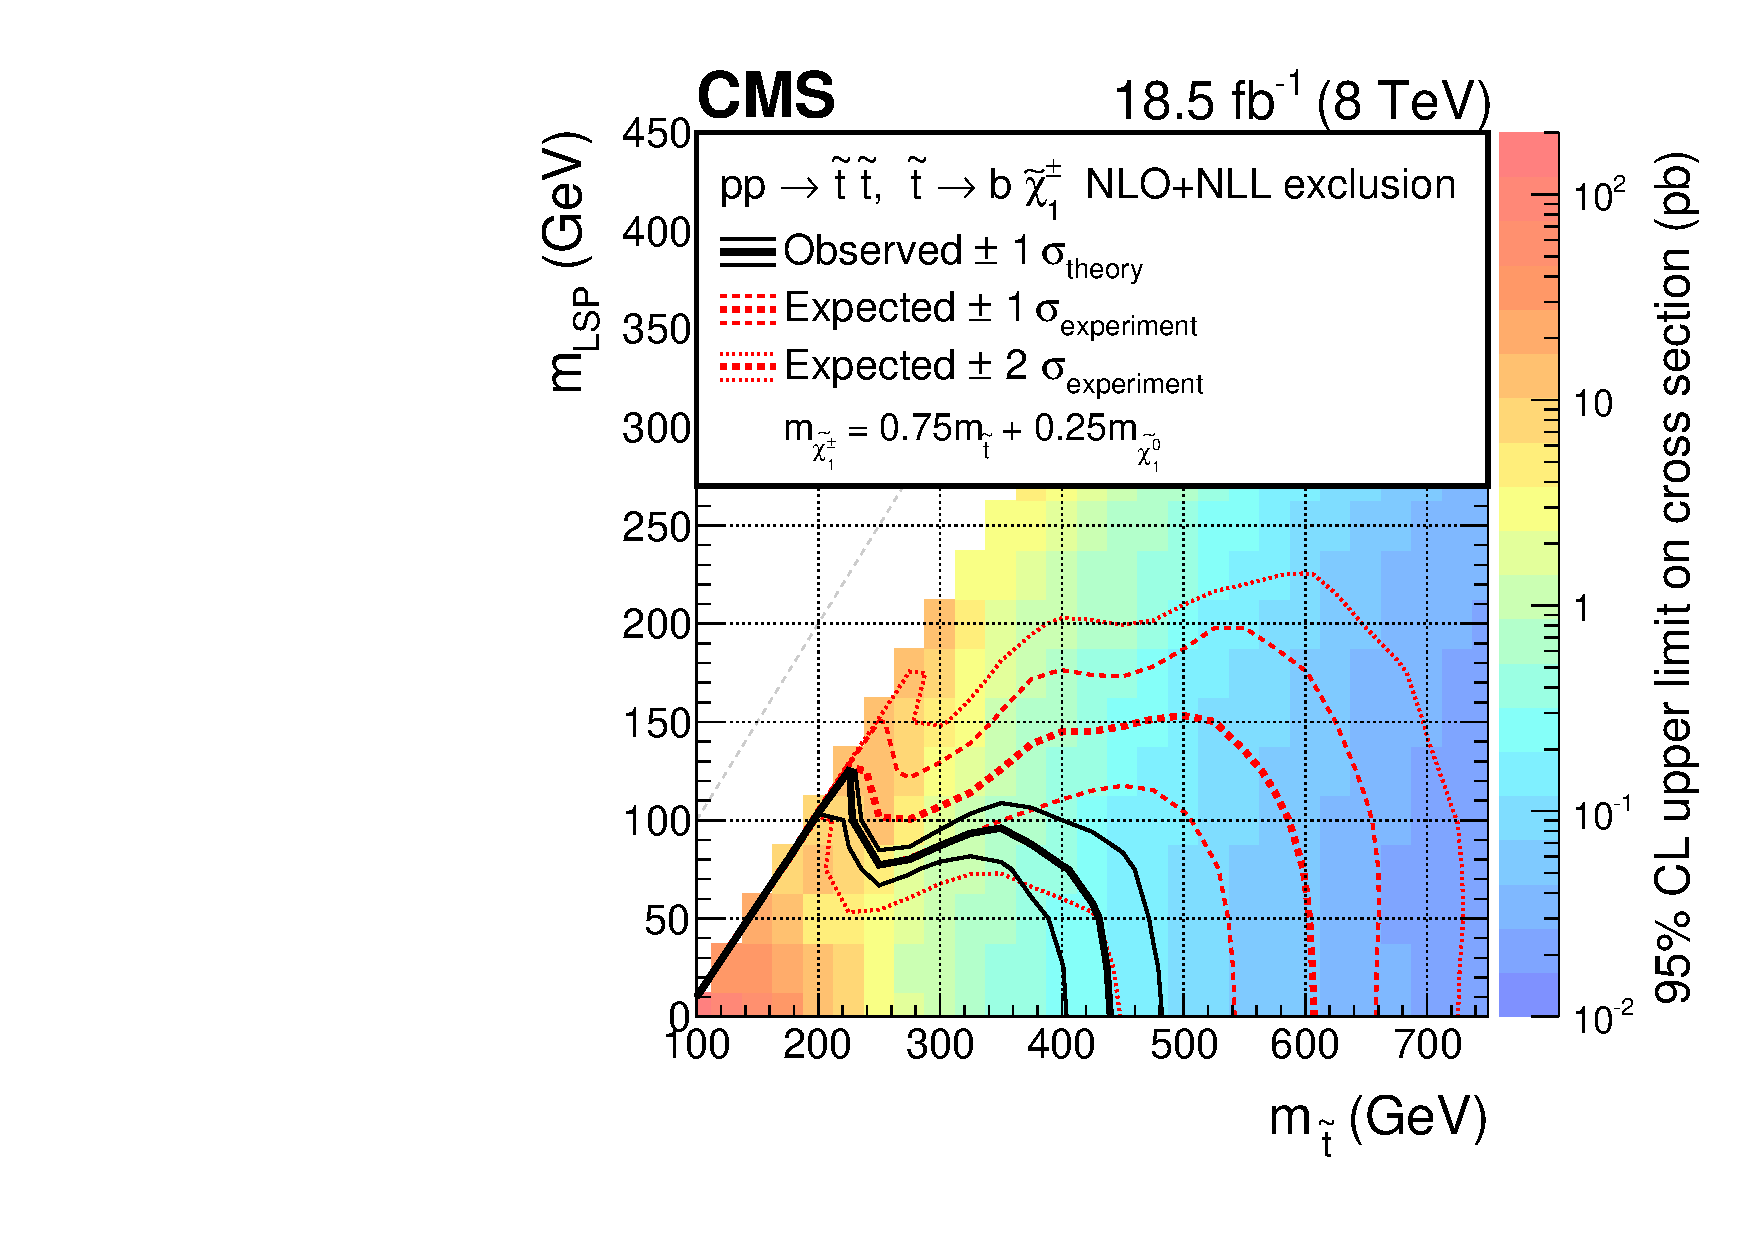
\includegraphics[width=0.40\textwidth]{Figure_003-d.pdf}
      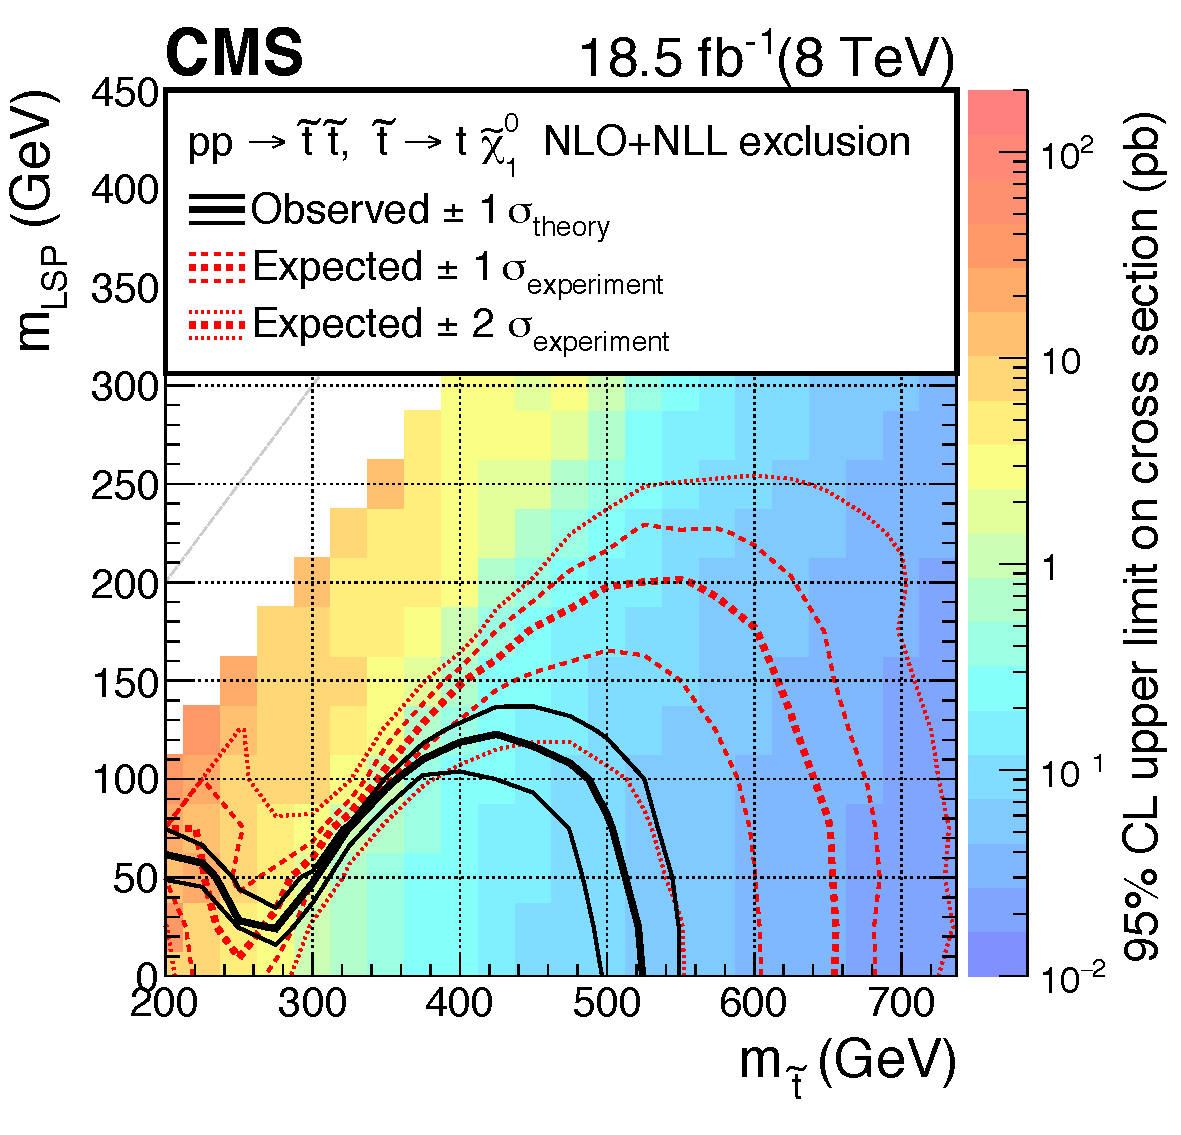
\includegraphics[width=0.40\textwidth]{Figure_003-e.pdf}
      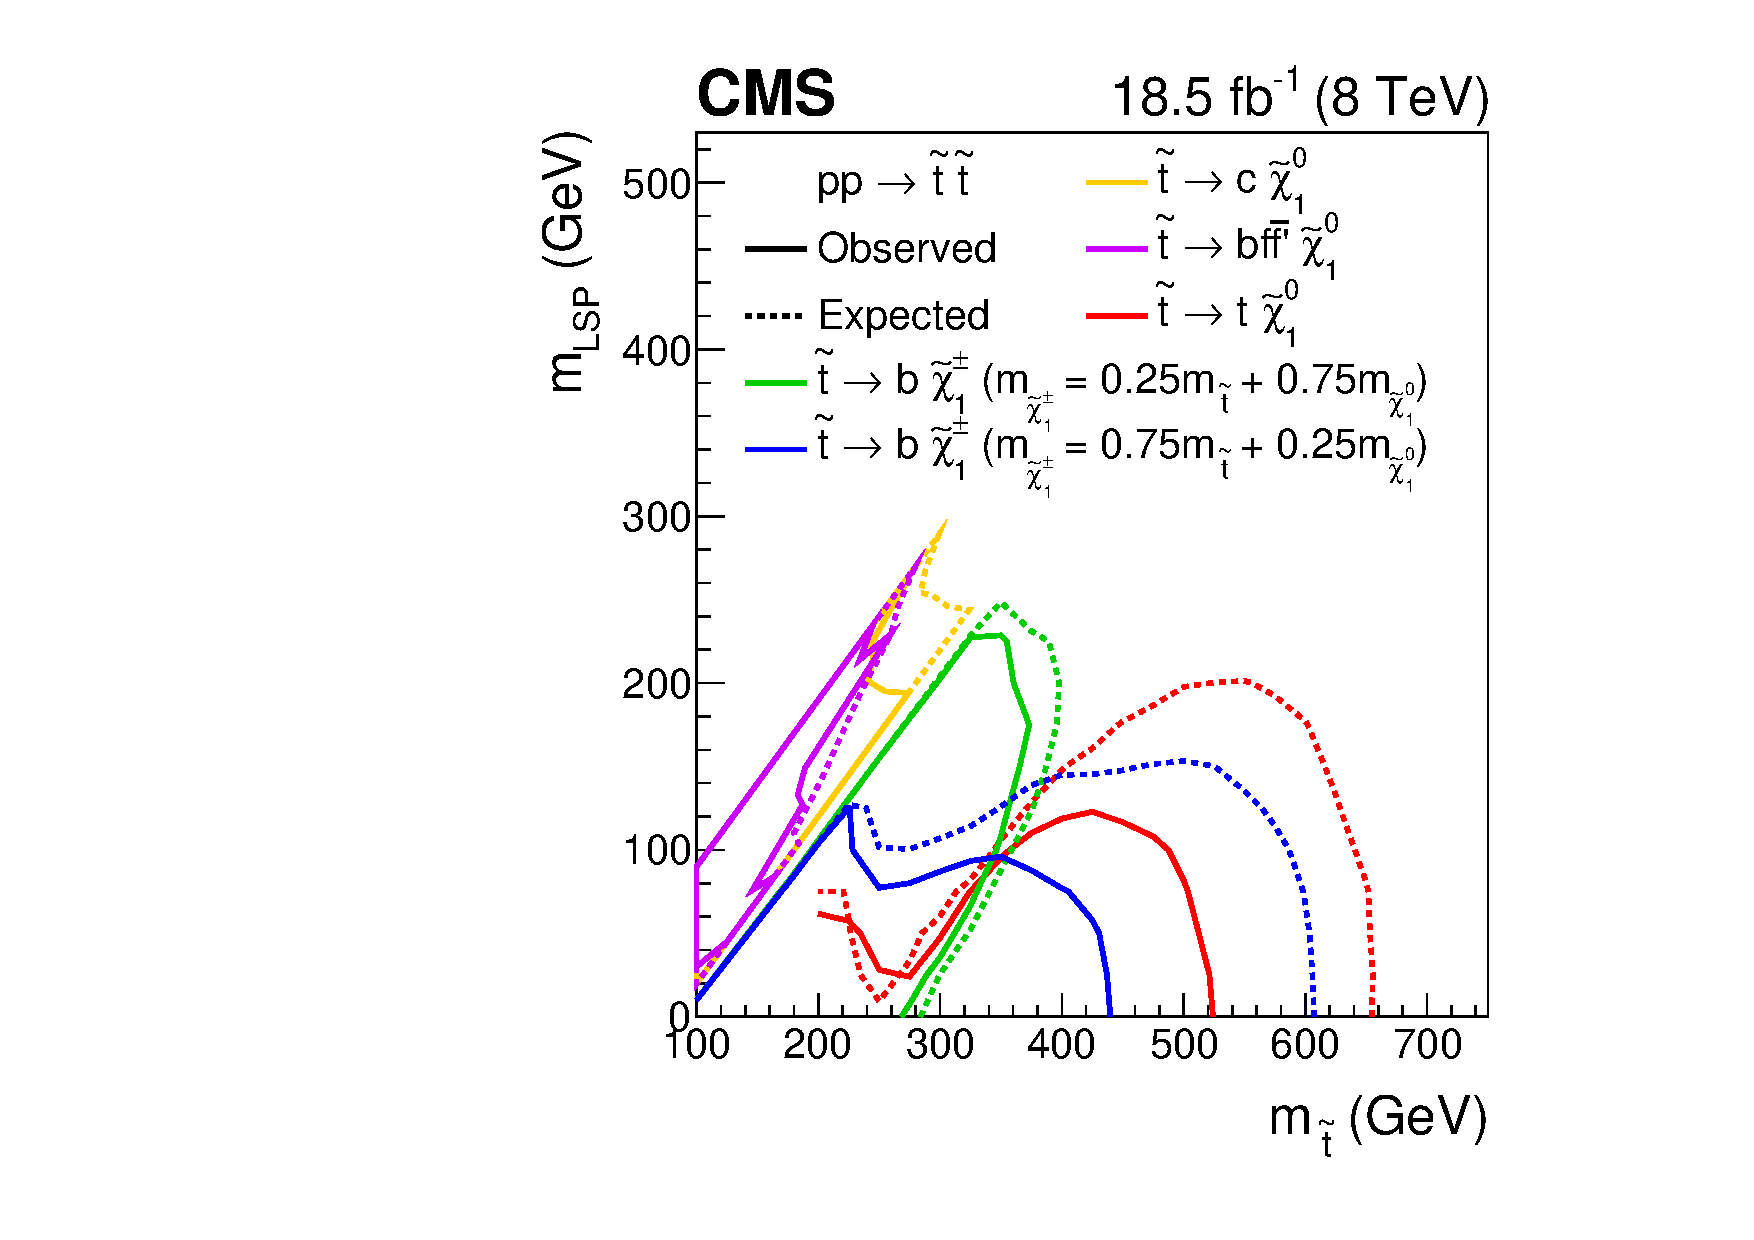
\includegraphics[width=0.40\textwidth]{Figure_003-f.pdf}
    \caption{ Observed upper limits on the production cross section at
      95\% CL (indicated by the colour scale) as a function of the
      top squark and $\PSGczDo$ masses for
      (upper left) $\PSQt \to\PQc\PSGczDo$,
      (upper right) $\PSQt \to{\PQb \ffbp}\PSGczDo$,
      (middle left) $\PSQt \to\PQb\PSGcpmDo$ with $m_{\PSGcpmDo} = 0.25m_{\PSQt} + 0.75m_{\PSGczDo}$,
      (middle right) $\PSQt \to\PQb\PSGcpmDo$ with $m_{\PSGcpmDo} = 0.75m_{\PSQt} + 0.25m_{\PSGczDo}$, and
      (lower left) $\PSQt \to\PQt \PSGczDo$.
      The black solid thick curves indicate the observed exclusion
      assuming the NLO+NLL SUSY production cross sections; the thin
      black curves show corresponding ${\pm}1\sigma$ theoretical
      uncertainties. The red thick dashed curves indicate median
      expected exclusions and the thin dashed and dotted
      curves indicate, respectively, their ${\pm}1 \sigma$ and
      ${\pm}2\sigma$ experimental uncertainties. A summary of the
      observed (solid) and median expected (dotted) exclusion contours
      is presented (lower right). The grey dotted diagonal lines
      delimit the region for which $m_{\PSQt} > m_{\PSGczDo}$.
      \label{fig:limits-sms}
    }
\end{figure*}

Figure~\ref{fig:limits-sms} shows the observed upper limit on the
production cross section at 95\% confidence level (CL), as a function
of the top squark and $\PSGczDo$ masses, for a range of simplified
models based on the pair production of top squarks, together with
excluded mass regions.

Figures~\ref{fig:limits-sms} (upper left and right) show the
sensitivity of this analysis to the decay modes $\PSQt \to
\PQc\PSGczDo$ and $\PSQt \to\PQb \ffbp \PSGczDo$, respectively.  The
excluded regions are determined using the NLO+NLL cross sections for
top squark pair production, assuming that b squarks, light-flavoured
squarks, and gluinos are too heavy to be produced in the pp
collisions. Also shown are the excluded regions observed when the
production cross section is changed by its theoretical uncertainty,
and the expected region of exclusion, as well as those determined for
both ${\pm}1$ and ${\pm}2$ standard deviation ($\sigma$) changes in
experimental uncertainties. The range of excluded top squark masses is
sensitive to both the decay mode and \dm. For the decay $\PSQt
\to\PQc\PSGczDo$, the excluded region is relatively stable as a
function of \dm, with $\PSQt$ masses below 285 and 325\GeV excluded,
respectively, for $\dm = 10$ and 80\GeV. The observed exclusion,
assuming the theoretical production cross section reduced by its
$1\sigma$ uncertainty, is weaker, with $\PSQt$ masses below 240 and
260\GeV excluded for $\dm = 10$ and 80\GeV. For the decay $\PSQt
\to\PQb \ffbp \PSGczDo$, the expected excluded mass region is strongly
dependent on \dm, weakening considerably for increasing values of \dm
due to the increased momentum phase space available to leptons
produced in the four-body decay. Top squark masses below 265 and
165\GeV are excluded based on the expected results, respectively, for
$\dm = 10$ and 80\GeV. The observed exclusion is again weaker, with
masses below 230 and 130\GeV excluded. The nonsmooth behaviour of the
exclusion contours is the result of statistical fluctuations and the
sparseness of the scan over the mass parameter space, and does not
represent a kinematical effect.

Figures~\ref{fig:limits-sms} (middle left and right) show the limits
on the allowed cross section for the decay $\PSQt \to \PQb \PSGcpmDo$,
followed by a decay of the $\PSGcpmDo$ to the $\PSGczDo$ and to either
an on- or off-shell W boson, depending on the mass difference between
the $\PSGcpmDo$ and $\PSGczDo$.  For a model with $m_{\PSGcpmDo} =
0.25m_{\PSQt} + 0.75m_{\PSGczDo}$, shown in Fig.~\ref{fig:limits-sms}
(middle left), the analysis has sensitivity in the region
$m_{\PSGcpmDo} - m_{\PSGczDo} < m_{\PW}$, excluding $\PSGczDo$ masses
up to $225 \GeV$ and $\PSQt$ masses up to $260 \GeV$. For a model with
$m_{\PSGcpmDo} = 0.75m_{\PSQt} + 0.25m_{\PSGczDo}$, shown in
Fig.~\ref{fig:limits-sms} (middle right), $\PSQt$ masses up to $400
\GeV$ can be excluded but the reach in $\PSGczDo$ mass is reduced.

Figure~\ref{fig:limits-sms} (lower left) shows the results of the
analysis for the decay $\PSQt \to \PQt \PSGczDo$,
where $\PSQt$ masses up to $500 \GeV$ are excluded.  As in
Fig.~\ref{fig:limits-sms} (middle right), the observed limit is around
2$\sigma$ below the expected result for large values of
$m_{\PSQt}$. This is mainly due to an excess of observed counts in
data in the $\nb=2$ categories in the region of $500 < \scalht < 700
\GeV$, which is compatible with a statistical fluctuation.  The
observed limits lie closer to the expected values at low top squark
masses, which correspond to lower values of \scalht for which good
agreement between the data and SM background predictions is observed.

Figure~\ref{fig:limits-sms} (lower right) presents a summary of all
the expected and observed exclusion contours and indicates that the
analysis has good sensitivity across many different decay signatures
in the $m_{\PSQt}$--$m_{\PSGczDo}$ plane.

\section{Summary}

An inclusive search for supersymmetry with the CMS detector is
reported, based on data from pp collisions collected at $\sqrt{s} =
8\TeV$, corresponding to an integrated luminosity of $18.5 \pm 0.5
\fbinv$. The final states analysed contain two or more jets with large
transverse energies and a significant imbalance in the event
transverse momentum, as expected in the production and decay of
massive squarks and gluinos. Dedicated triggers made it possible to
extend the phase space covered in this search to values of \scalht and
\HTmiss as low as 200 and 130\GeV, respectively.  These regions of low
\scalht and \HTmiss correspond to regions of phase space that are
highly populated in models with low-mass squarks and nearly degenerate
mass spectra. The signal region is binned according to \scalht, the
number of reconstructed jets, and the number of jets identified as
originating from b quarks. The sum of standard model backgrounds in
each bin is estimated from a simultaneous binned likelihood fit to the
event yields in the signal region and in \mj, \mmj, and \gj control
samples. The observed yields in the signal region are found to be in
agreement with the expected contributions from standard model
processes.

Limits are determined in the mass parameter space of simplified models
that assume the direct pair production of top squarks. A comprehensive
study of top squark decay modes is performed and interpreted in the
parameter space of the loop-induced two-body decays to the neutralino
and one c quark ($\PSQt \to \PQc\PSGczDo$); four-body decays to the
neutralino, one b quark, and an off-shell W boson ($\PSQt \to {\PQb
  \ffbp} \PSGczDo$); decays to one b quark and the lightest chargino
($\PSQt \to \PQb \PSGcpmDo$), followed by the decay of the chargino to
the lightest neutralino and an (off-shell) W boson; and the decay to a
top quark and neutralino ($\PSQt \to \PQt \PSGczDo$). In the region
$m_{\PSQt} - m_{\PSGczDo} < m_{\PW}$, top squarks with masses as large
as 260 and 230\GeV, and neutralino masses up to 240 and 220\GeV, are
excluded, respectively, for the two- and four-body decay modes. For
top squark decays to $\PQb\PSGcpmDo$, top squark masses up to 400\GeV
and neutralino masses up to 225\GeV are excluded, depending on the
mass of the chargino. For top squarks decaying to a top quark and a
neutralino, top squark masses up to 500\GeV and neutralino masses up
to 105\GeV are excluded.

In summary, the analysis provides sensitivity across a large region of
parameter space in the ($m_{\PSQt}, m_{\PSGczDo}$) plane, covering
several relevant top squark decay modes. In particular, the
application of low thresholds to maximise signal acceptance provides
sensitivity to models with compressed mass spectra. For top squark
decays to b$\PSGcpmDo$, where the W boson from the $\PSGcpmDo$ decay
is off-shell, the presented studies improve on existing limits.  Mass
exclusions are reported in previously unexplored regions of the
$(m_{\PSQt}, m_{\PSGcpmDo}, m_{\PSGczDo})$ parameter space that
satisfy $100\GeV < \dm < m_\PQt$, of up to $m_{\PSQt} = 325$,
$m_{\PSGcpmDo} = 250$, and $m_{\PSGczDo} = 225\GeV$. For the region
$\dm < m_\PW$, the search provides the strongest expected mass
exclusions, up to $m_{\PSQt} = 325\GeV$, for the two-body decay $\PSQt
\to \PQc\PSGczDo$ when $30\GeV < \dm < m_\PW$.

\begin{acknowledgments}

  We congratulate our colleagues in the CERN accelerator departments
  for the excellent performance of the LHC and thank the technical and
  administrative staffs at CERN and at other CMS institutes for their
  contributions to the success of the CMS effort. In addition, we
  gratefully acknowledge the computing centres and personnel of the
  Worldwide LHC Computing Grid for delivering so effectively the
  computing infrastructure essential to our analyses. Finally, we
  acknowledge the enduring support for the construction and operation
  of the LHC and the CMS detector provided by the following funding
  agencies: BMWFW and FWF (Austria); FNRS and FWO (Belgium); CNPq,
  CAPES, FAPERJ, and FAPESP (Brazil); MES (Bulgaria); CERN; CAS, MoST,
  and NSFC (China); COLCIENCIAS (Colombia); MSES and CSF (Croatia);
  RPF (Cyprus); MoER, ERC IUT and ERDF (Estonia); Academy of Finland,
  MEC, and HIP (Finland); CEA and CNRS/IN2P3 (France); BMBF, DFG, and
  HGF (Germany); GSRT (Greece); OTKA and NIH (Hungary); DAE and DST
  (India); IPM (Iran); SFI (Ireland); INFN (Italy); MSIP and NRF
  (Republic of Korea); LAS (Lithuania); MOE and UM (Malaysia); BUAP,
  CINVESTAV, CONACYT, LNS, SEP, and UASLP-FAI (Mexico); MBIE (New
  Zealand); PAEC (Pakistan); MSHE and NSC (Poland); FCT (Portugal);
  JINR (Dubna); MON, RosAtom, RAS and RFBR (Russia); MESTD (Serbia);
  SEIDI and CPAN (Spain); Swiss Funding Agencies (Switzerland); MST
  (Taipei); ThEPCenter, IPST, STAR and NSTDA (Thailand); TUBITAK and
  TAEK (Turkey); NASU and SFFR (Ukraine); STFC (United Kingdom); DOE
  and NSF (USA).

  Individuals have received support from the Marie-Curie programme and
  the European Research Council and EPLANET (European Union); the
  Leventis Foundation; the A. P. Sloan Foundation; the Alexander von
  Humboldt Foundation; the Belgian Federal Science Policy Office; the
  Fonds pour la Formation \`a la Recherche dans l'Industrie et dans
  l'Agriculture (FRIA-Belgium); the Agentschap voor Innovatie door
  Wetenschap en Technologie (IWT-Belgium); the Ministry of Education,
  Youth and Sports (MEYS) of the Czech Republic; the Council of
  Science and Industrial Research, India; the HOMING PLUS programme of
  the Foundation for Polish Science, cofinanced from European Union,
  Regional Development Fund; the Mobility Plus programme of the
  Ministry of Science and Higher Education (Poland); the OPUS
  programme of the National Science Center (Poland); the Thalis and
  Aristeia programmes cofinanced by EU-ESF and the Greek NSRF; the
  National Priorities Research Program by Qatar National Research
  Fund; the Programa Clar\'in-COFUND del Principado de Asturias; the
  Rachadapisek Sompot Fund for Postdoctoral Fellowship, Chulalongkorn
  University (Thailand); the Chulalongkorn Academic into Its 2nd
  Century Project Advancement Project (Thailand); and the Welch
  Foundation, contract C-1845.

\end{acknowledgments}

\bibliography{auto_generated}
